\documentclass[
	letterpaper, % Paper size, specify a4paper (A4) or letterpaper (US letter)
	10pt, % Default font size, specify 10pt, 11pt or 12pt
]{CSUniSchoolLabReport}

%----------------------------------------------------------------------------------------
%	REPORT INFORMATION
%----------------------------------------------------------------------------------------

\title{Seven-Segment Display \\ Embedded Design: Enabling Robotics \\ EECE2160} % Report title

\author{Michael \textsc{Brodskiy}\\ \small \href{mailto:Brodskiy.M@Northeastern.edu}{Brodskiy.M@Northeastern.edu}}

\date{February 9, 2023} % Date of the report

%----------------------------------------------------------------------------------------


\begin{document}

\maketitle % Insert the title, author and date using the information specified above

\begin{center}
	\begin{tabular}{l r}
		Date Performed: & February 2, 2023 \\ % Date the experiment was performed
        Partner: & Dylan \textsc{Powers} \\ % Partner names
		Instructor: & Professor \textsc{Shazli} % Instructor/supervisor
	\end{tabular}
\end{center}

\newpage

\begin{abstract}

  The purpose of this laboratory experimentation is to fabricate and understand the process of digital logic circuits. This laboratory procedure allows for the formation of a deeper understanding of real-life digital logic applications through the integration of a seven-segment display. Optimally-minimized boolean equations were then constructed from Karnaugh maps to construct final circuit designs.

\end{abstract}

\begin{flushleft}

  \textsc{Keywords:} \underline{minimization}, \underline{boolean equation}, \underline{seven-segment display}, \underline{optimal}, \underline{Karnaugh map}

\end{flushleft}

\newpage

\section{Equipment}

\hspace{.5 in} Available equipment included:\\

\begin{itemize}

  \item DE1-SoC board

  \item DE1-SoC Power Cable

  \item USB-A to USB-B Cable

  \item Computer

  \item Quartus Prime Schematic Software

\end{itemize}

\section{Pre-Lab}

The pre-lab consisted of the construction of a truth table based on the provided scenario, as well as subsequent conversion to minimized boolean equations through the use of Karnaugh maps.

\subsection{Truth Table}

\begin{table}[H]
  \centering
  \begin{tabular}{| c || c | c | c | c || c | c | c | c | c | c | c |}
    \hline
    \# & In3 & In2 & In1 & In0 & a & b & c & d & e & f & g \\
    \hline
    0 & 0 & 0 & 0 & 0 & 0 & 0 & 0 & 0 & 0 & 0 & 1 \\
    \hline 
    1 & 0 & 0 & 0 & 1 & 1 & 0 & 0 & 1 & 1 & 1 & 1 \\
    \hline
    2 & 0 & 0 & 1 & 0 & 0 & 0 & 1 & 0 & 0 & 1 & 0 \\
    \hline
    3 & 0 & 0 & 1 & 1 & 0 & 0 & 0 & 0 & 1 & 1 & 0\\
    \hline
    4 & 0 & 1 & 0 & 0 & 1 & 0 & 0 & 1 & 1 & 0 & 0\\
    \hline
    5 & 0 & 1 & 0 & 1 & 0 & 1 & 0 & 0 & 1 & 0 & 0\\
    \hline
    6 & 0 & 1 & 1 & 0 & 0 & 1 & 0 & 0 & 0 & 0 & 0\\
    \hline
    7 & 0 & 1 & 1 & 1 & 0 & 0 & 0 & 1 & 1 & 1 & 1\\
    \hline
    8 & 1 & 0 & 0 & 0 & 0 & 0 & 0 & 0 & 0 & 0 & 0\\
    \hline
    9 & 1 & 0 & 0 & 1 & 0 & 0 & 0 & 0 & 1 & 0 & 0\\
    \hline
  \end{tabular}
  \caption{Digits to display on a 7-stage display (0 for on, 1 for off)}
  \label{tab:1}
\end{table}

\subsection{Karnaugh Maps}

    \begin{table}[H]
      \centering
      \begin{tabular}{|c | c | c | c | c |}
        \hline
        In3In2 | In1In0 & 00 & 01 & 11 & 10\\
        \hline
        00 & 0 & 1 & 0 & 0\\
        \hline
        01 & 1 & 0 & 0 & 0\\
        \hline
        11 & x & x & x & x\\
        \hline
        10 & 0 & 0 & x & x\\
        \hline
      \end{tabular}
      \caption{Karnaugh Map for A $\rightarrow$ In2In1'In0' + In3'In2'In1'In0}
      \label{tab:2}
    \end{table}

    \begin{table}[H]
      \centering
      \begin{tabular}{|c | c | c | c | c |}
        \hline
        In3In2 |  In1In0 & 00 & 01 & 11 & 10\\
        \hline
        00 & 0 & 0 & 0 & 0\\
        \hline
        01 & 0 & 1 & 0 & 1\\
        \hline
        11 & x & x & x & x\\
        \hline
        10 & 0 & 0 & x & x\\
        \hline
      \end{tabular}
      \caption{Karnaugh Map for B $\rightarrow$ In2In1'In0 + In2In1In0'}
      \label{tab:3}
    \end{table}

    \begin{table}[H]
      \centering
      \begin{tabular}{|c | c | c | c | c |}
        \hline
        In3In2 |  In1In0 & 00 & 01 & 11 & 10\\
        \hline
        00 & 0 & 0 & 0 & 1\\
        \hline
        01 & 0 & 0 & 0 & 0\\
        \hline
        11 & x & x & x & x\\
        \hline
        10 & 0 & 0 & x & x\\
        \hline
      \end{tabular}
      \caption{Karnaugh Map for C $\rightarrow$ In3'In2'In1In0'}
      \label{tab:4}
    \end{table}

    \begin{table}[H]
      \centering
      \begin{tabular}{|c | c | c | c | c |}
        \hline
        In3In2 |  In1In0 & 00 & 01 & 11 & 10\\
        \hline
        00 & 0 & 1 & 0 & 0\\
        \hline
        01 & 1 & 0 & 1 & 0\\
        \hline
        11 & x & x & x & x\\
        \hline
        10 & 0 & 0 & x & x\\
        \hline
      \end{tabular}
      \caption{Karnaugh Map for D $\rightarrow$ In2In1'In0' + In3'In2'In1'In0 + In2In1In0}
      \label{tab:5}
    \end{table}

    \begin{table}[H]
      \centering
      \begin{tabular}{|c | c | c | c | c |}
        \hline
        In3In2 |  In1In0 & 00 & 01 & 11 & 10\\
        \hline
        00 & 0 & 1 & 1 & 0\\
        \hline
        01 & 1 & 1 & 1 & 0\\
        \hline
        11 & x & x & x & x\\
        \hline
        10 & 0 & 1 & x & x\\
        \hline
      \end{tabular}
      \caption{Karnaugh Map for E $\rightarrow$ In2In1'In0' + In0}
      \label{tab:6}
    \end{table}

    \begin{table}[H]
      \centering
      \begin{tabular}{|c | c | c | c | c |}
        \hline
        In3In2 |  In1In0 & 00 & 01 & 11 & 10\\
        \hline
        00 & 0 & 1 & 1 & 1\\
        \hline
        01 & 0 & 0 & 1 & 0\\
        \hline
        11 & x & x & x & x\\
        \hline
        10 & 0 & 0 & x & x\\
        \hline
      \end{tabular}
      \caption{Karnaugh Map for F $\rightarrow$ In3'In2'In0 + In3'In2'In1 + In1In0}
      \label{tab:7}
    \end{table}

    \begin{table}[H]
      \centering
      \begin{tabular}{|c | c | c | c | c |}
        \hline
        In3In2 |  In1In0 & 00 & 01 & 11 & 10\\
        \hline
        00 & 1 & 1 & 0 & 0\\
        \hline
        01 & 0 & 0 & 1 & 0\\
        \hline
        11 & x & x & x & x\\
        \hline
        10 & 0 & 0 & x & x\\
        \hline
      \end{tabular}
      \caption{Karnaugh Map for G $\rightarrow$ In3'In2'In1' + In2In1In0}
      \label{tab:8}
    \end{table}

\section{Introduction}

\hspace{.5 in} This lab revolved around the concept of seven-segment display integration. Displays consist of seven segments (thus the name), labeled A-G. Activating a certain sequence of these segments will result in the display of a certain number. Using the truth table, Karnaugh maps, and boolean equations generated in the pre-lab, this lab will concern the formation of a schematic to display a certain 4-bit number.\\

\hspace{.5 in} First and foremost, the aforementioned boolean equations were used to fully construct a seven-segment display digital logic circuit. This logic circuit was first functionally simulated, and then tested by flipping various combinations of switches to reach a desired output.\\

\hspace{.5 in} Next, some additional logic was added to the circuit, as an extra switch, which turned the seven-segment display on or off, was added. When on, this switch would activate the display, and display numbers as usual. When off, the switch dims the display, and nothing is displayed no matter the combination of number switches used.

\hspace{.5 in} As a final step, the concept of the control switch was applied to each of the 6 seven-segment displays present of the DE1-SoC board, allowing for the displays to show the same number on up to 6 displays, if all of the switches were to be turned on. Each display was controlled by the switch directly below it.

\section{Discussion \& Analysis} 

\subsection{Assignment 1}

\hspace{.5 in} The first of the assignments concerned the creation of the initial digital logic circuit. First and foremost, the equations derived in Tables \ref{tab:1}-\ref{tab:8} were combined to create one big circuit. This circuit is shown in Figure \ref{fig:1}. Prior to compiling and uploading to the board, a functional simulation was run to confirm the accuracy of the circuit, which was correct. The results of the simulation are shown in Figure \ref{fig:2}

\begin{figure}[H]
  \centering
  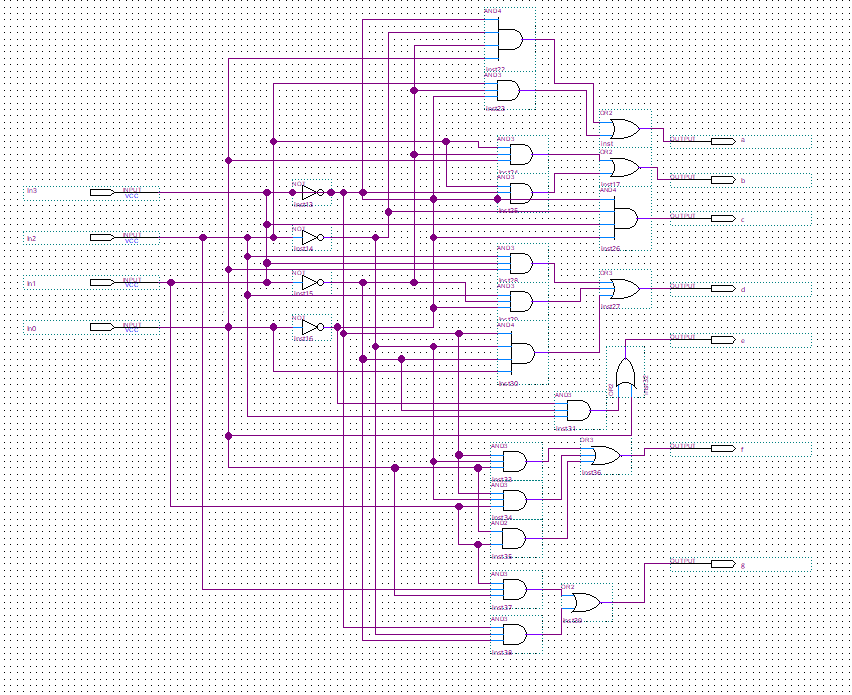
\includegraphics[width=.9\textwidth]{Figures/Design.png}
  \caption{The Seven-Segment Single-Control Circuit}
  \label{fig:1}
\end{figure}

\begin{figure}[H]
  \centering
  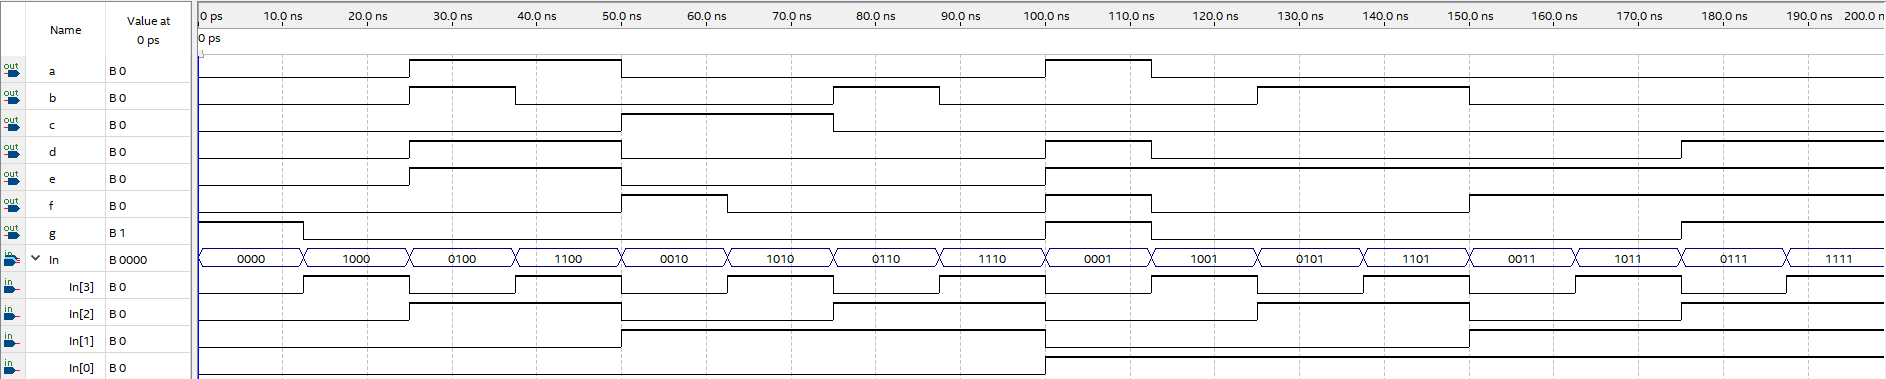
\includegraphics[width=.9\textwidth]{Figures/Sim.png}
  \caption{The Seven-Segment Single-Control Circuit Simulation}
  \label{fig:2}
\end{figure}

\subsection{Assignment 2}

\hspace{.5 in} For this assignment, the BCD system based on the derived Boolean equations created in Assignment 1 were uploaded to the DE1-SoC board for testing on the first 7-digit display (HEX0). When  assigning pins, the first for switches SW[3] (PIN\_AF10), SW[2] (PIN\_AF9), SW[1] (PIN\_AC12), and SW[0] (PIN\_AB12) were assigned to be the four inputs into the system IN3, IN2, IN1, and IN0 respectively. As for the outputs (a, b, c, d, e, f, g), these were assigned to HEX0[0] (PIN\_AE26), HEX0[1] (PIN\_AE27), HEX0[2] (PIN\_AE28), HEX0[3] (PIN\_AG27),  HEX0[4] (PINAF\_28), HEX0[5] (PIN\_AG28), and HEX0[6] (PIN\_AH28). The results of the testing on the DE1-SoC are shown in Figures \ref{fig:3}-\ref{fig:12} below.

\begin{figure}[H]
  \centering
  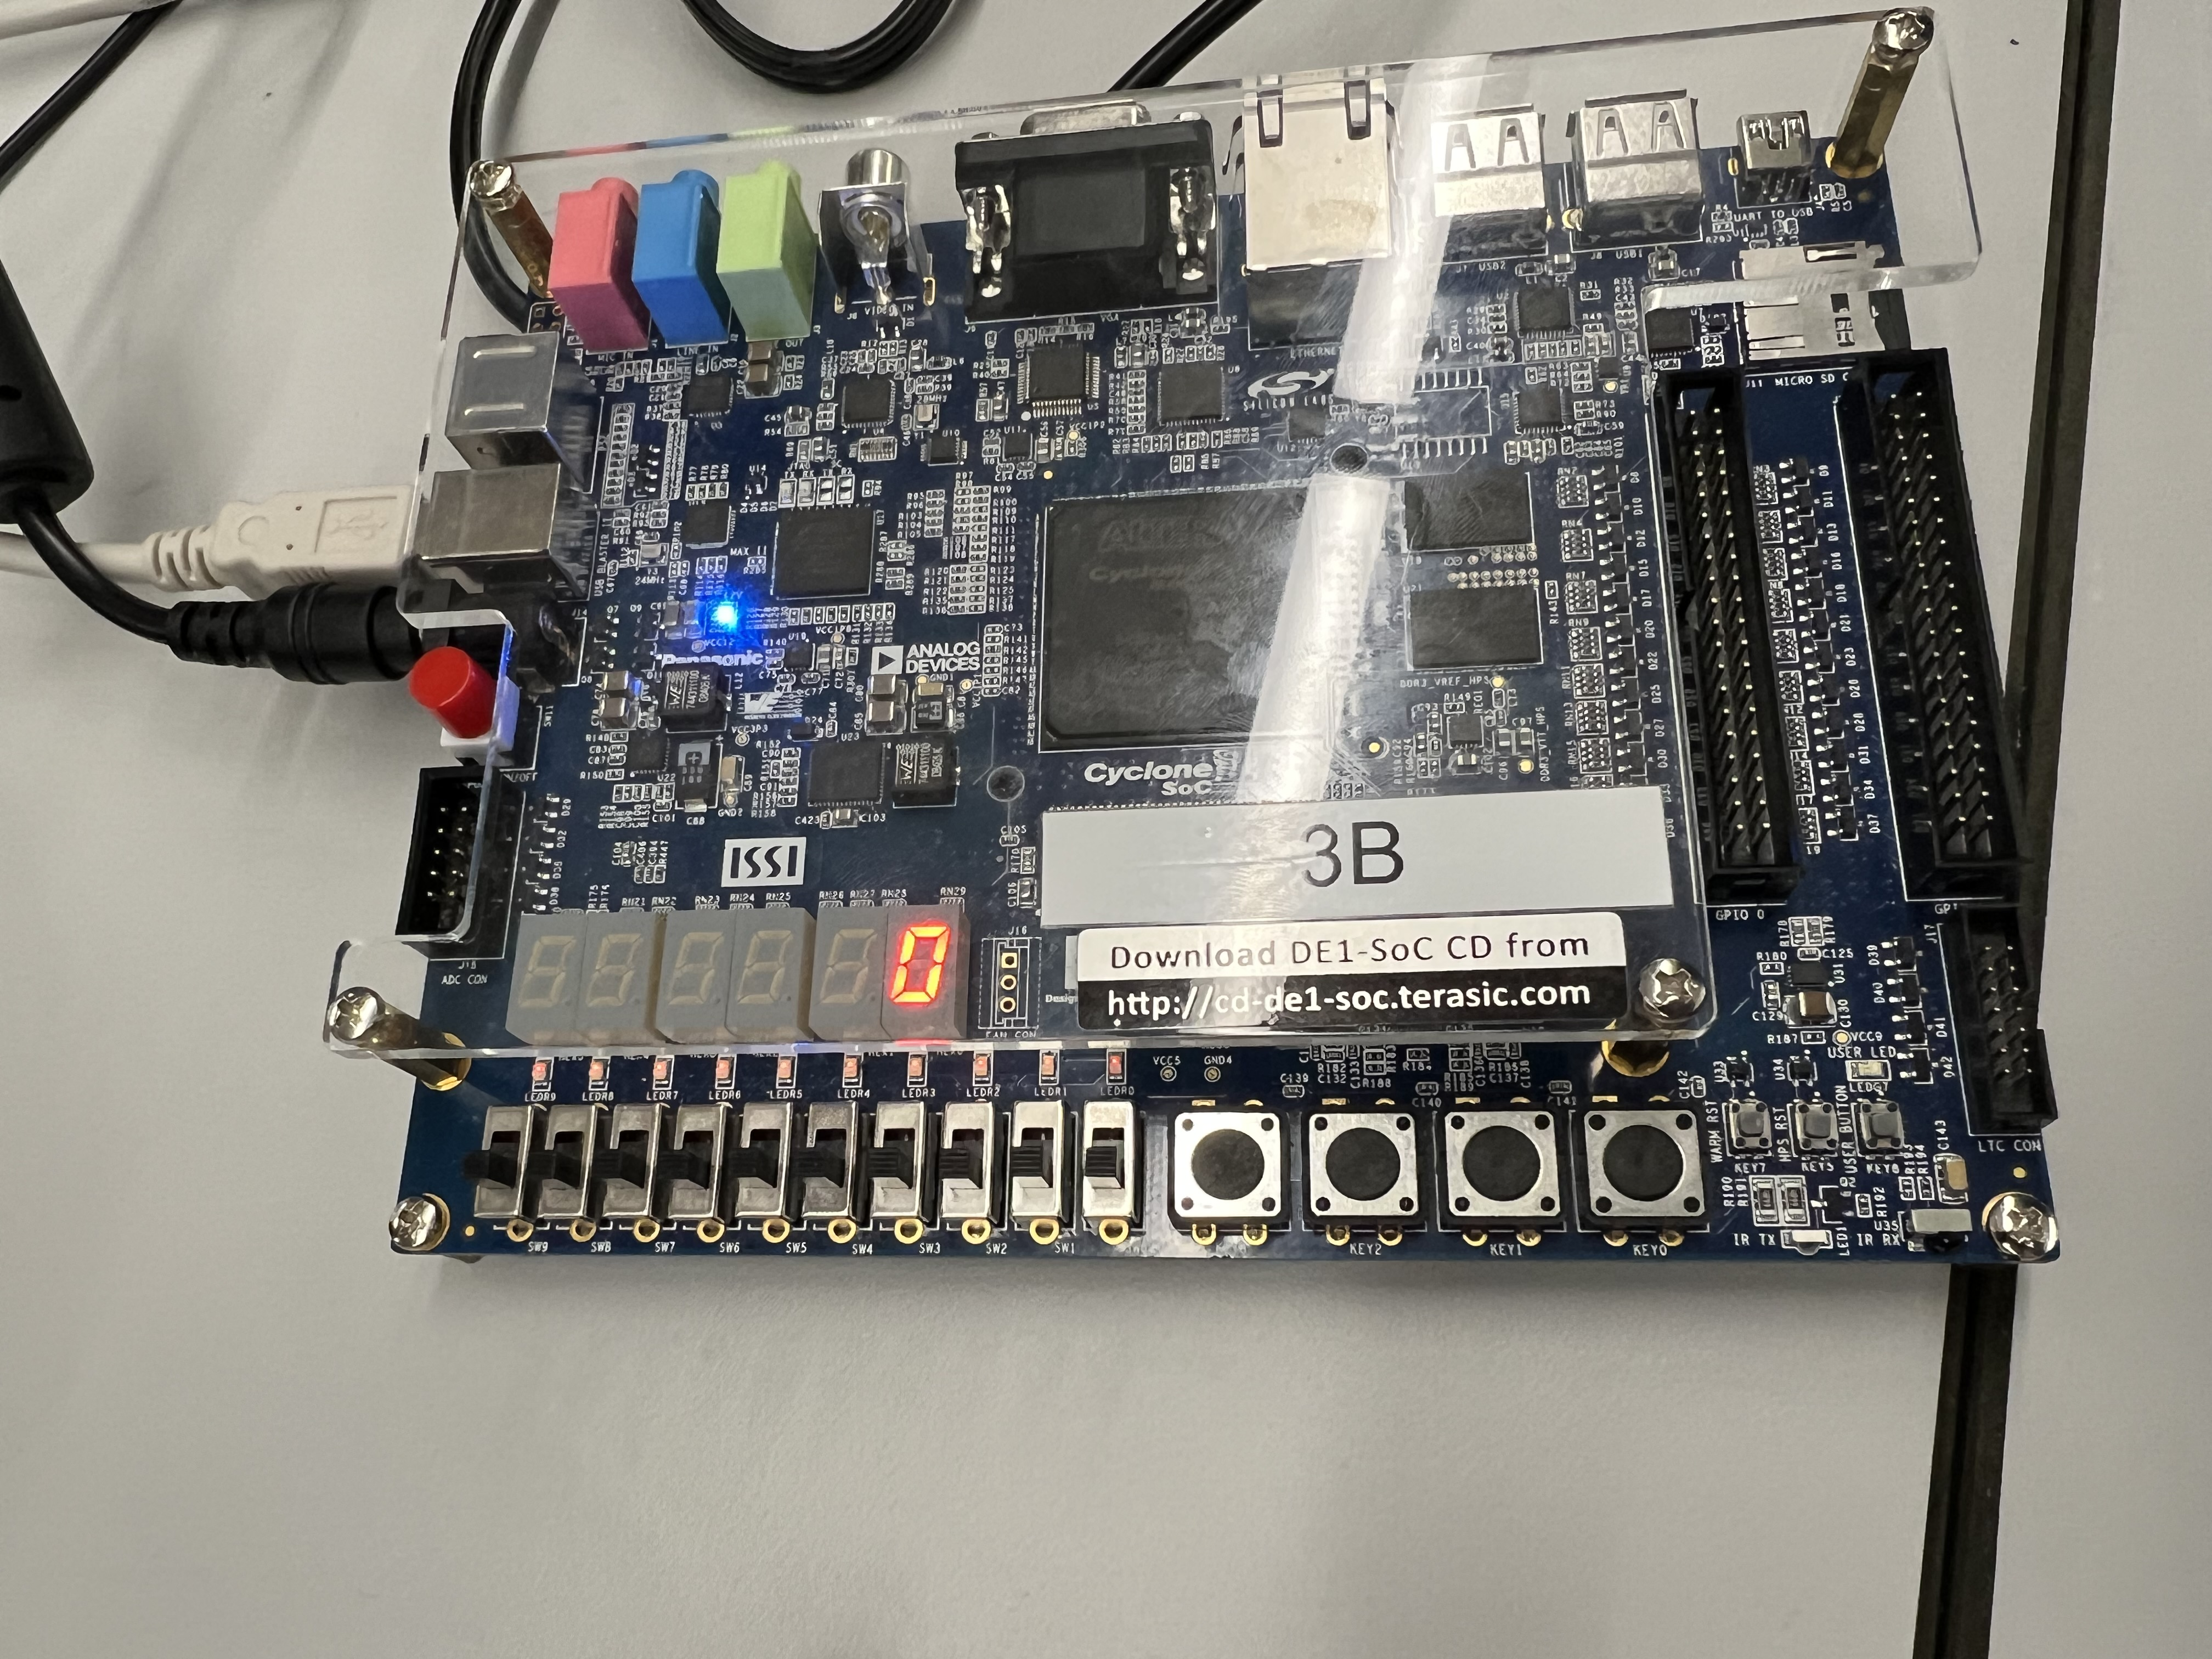
\includegraphics[width=.9\textwidth]{Figures/Disp_0.jpg}
  \caption{DE1-SoC Displaying 0 on HEX0 with no inputs}
  \label{fig:3}
\end{figure}

\begin{figure}[H]
  \centering
  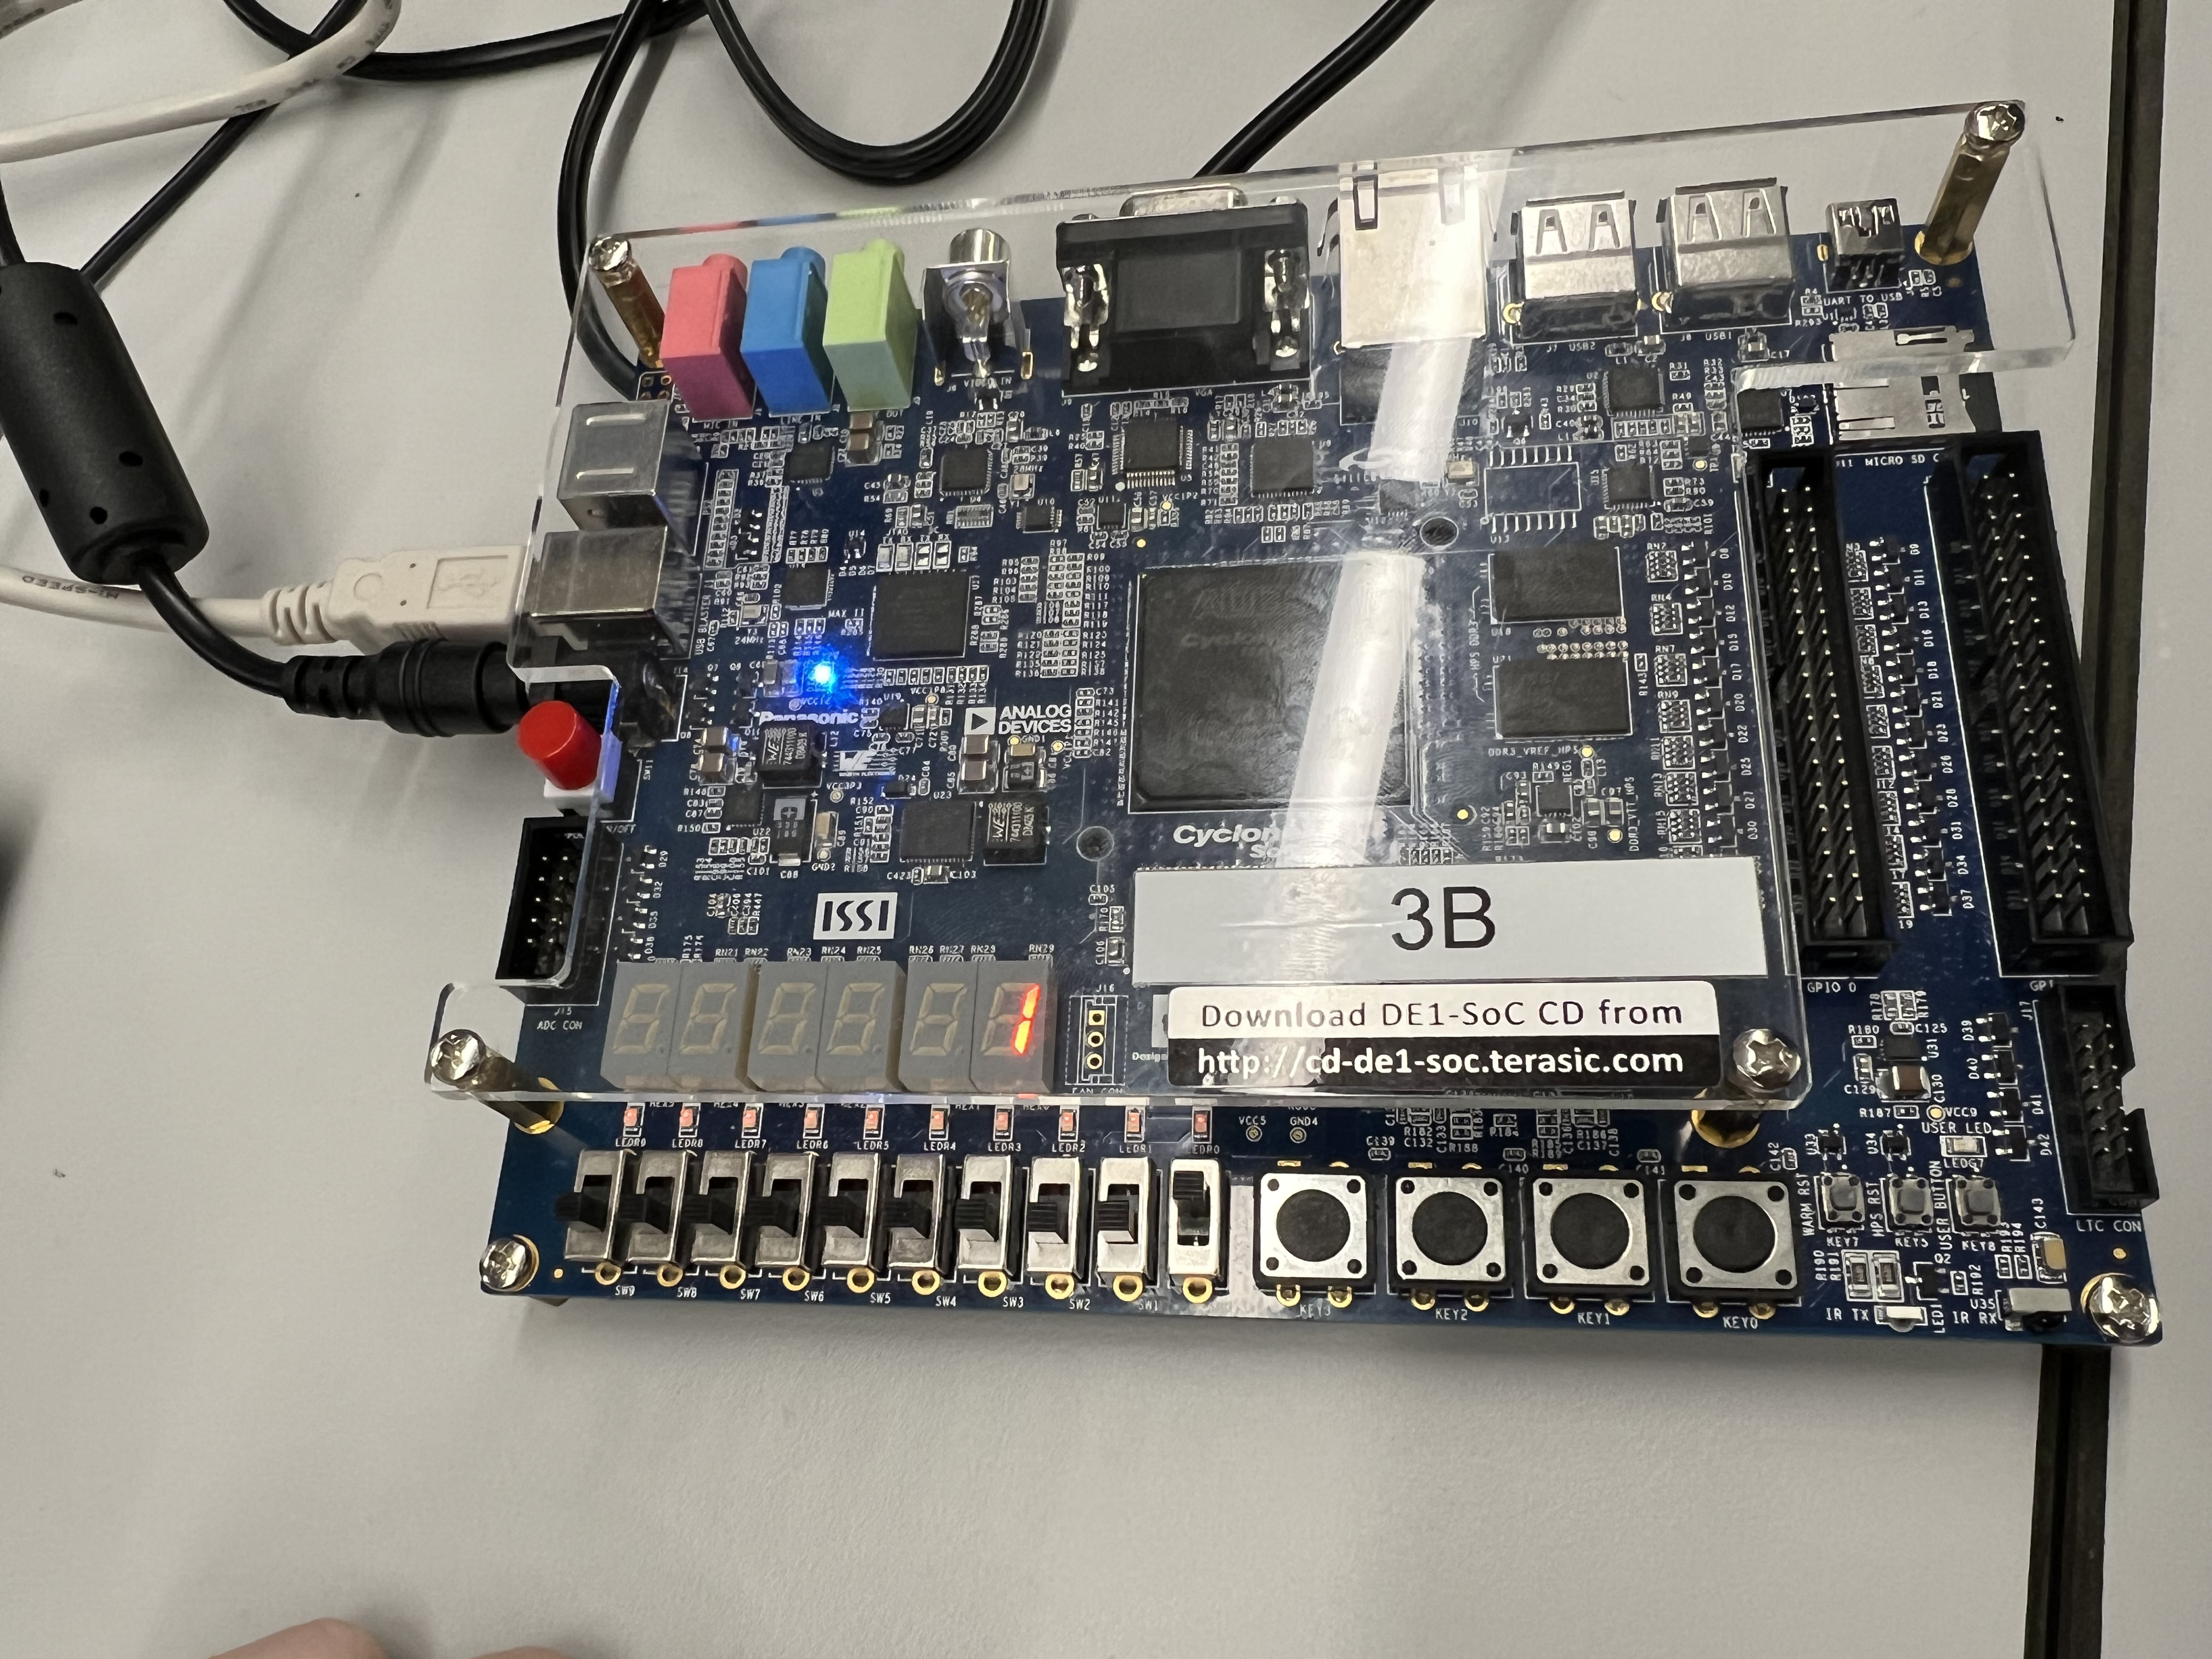
\includegraphics[width=.9\textwidth]{Figures/Disp_1.jpg}
  \caption{DE1-SoC Displaying 1 on HEX0 with input IN0}
  \label{fig:4}
\end{figure}

\begin{figure}[H]
  \centering
  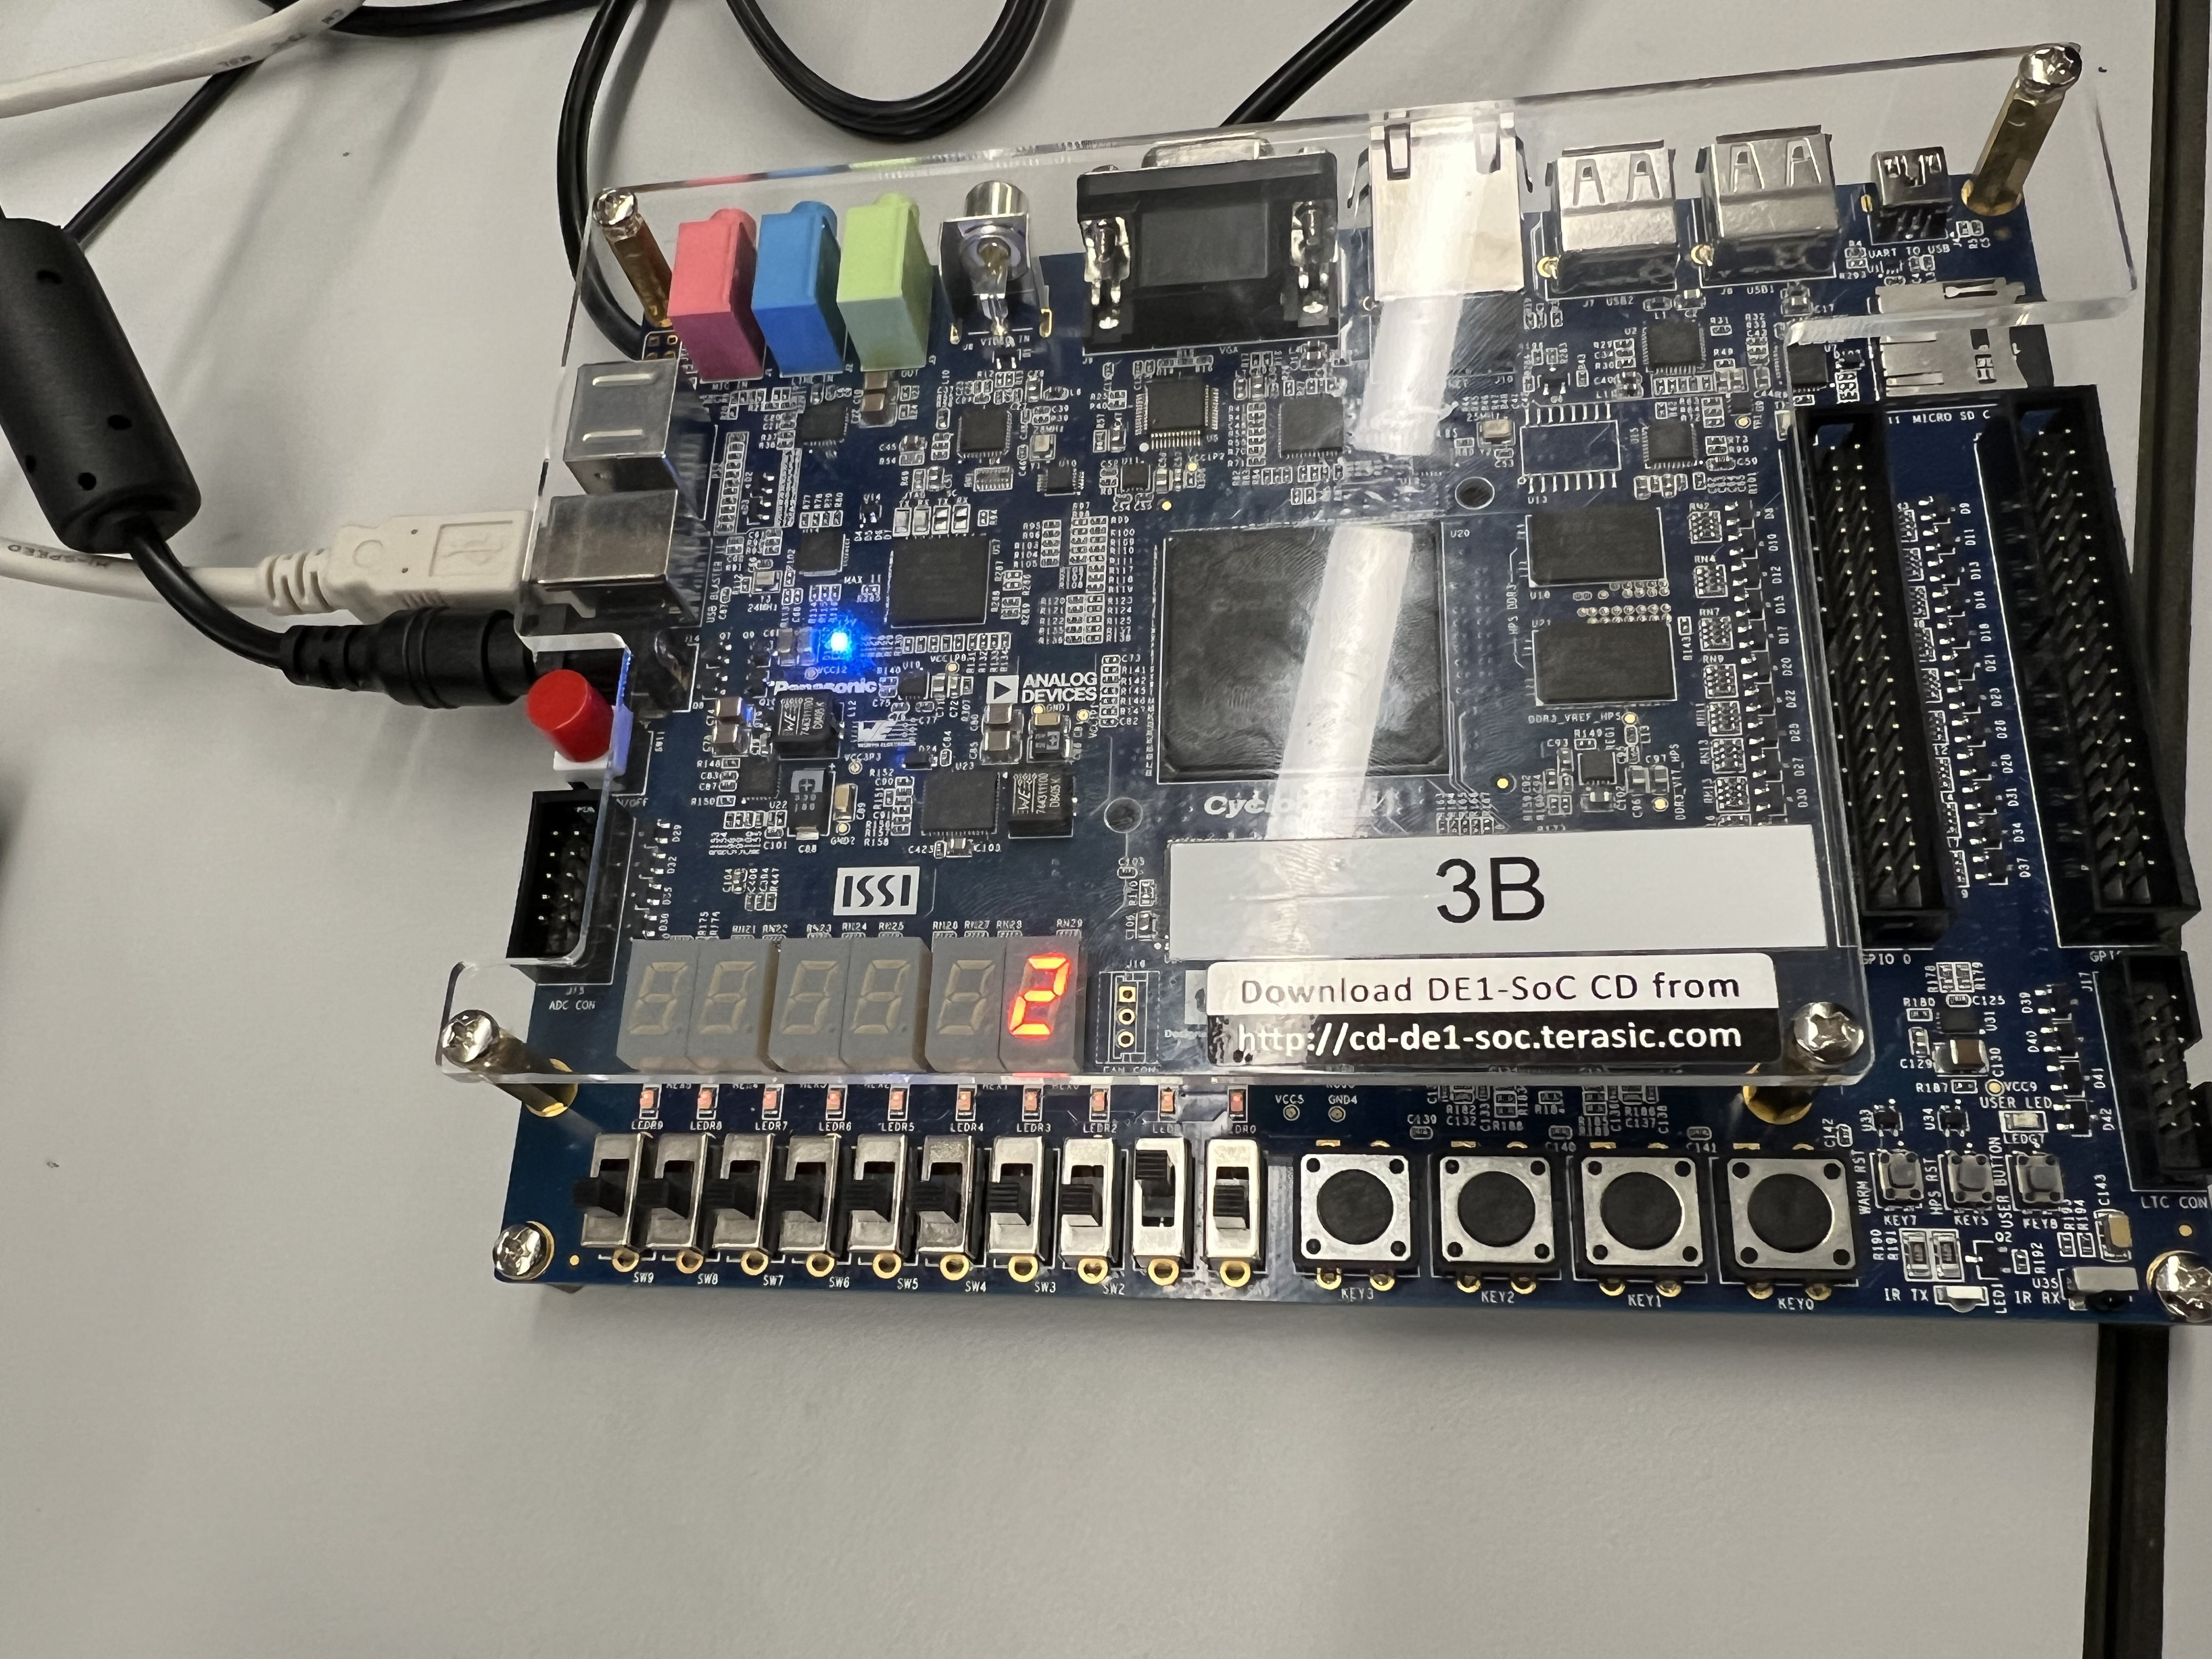
\includegraphics[width=.9\textwidth]{Figures/Disp_2.jpg}
  \caption{DE1-SoC Displaying 2 on HEX0 with input IN1}
  \label{fig:5}
\end{figure}

\begin{figure}[H]
  \centering
  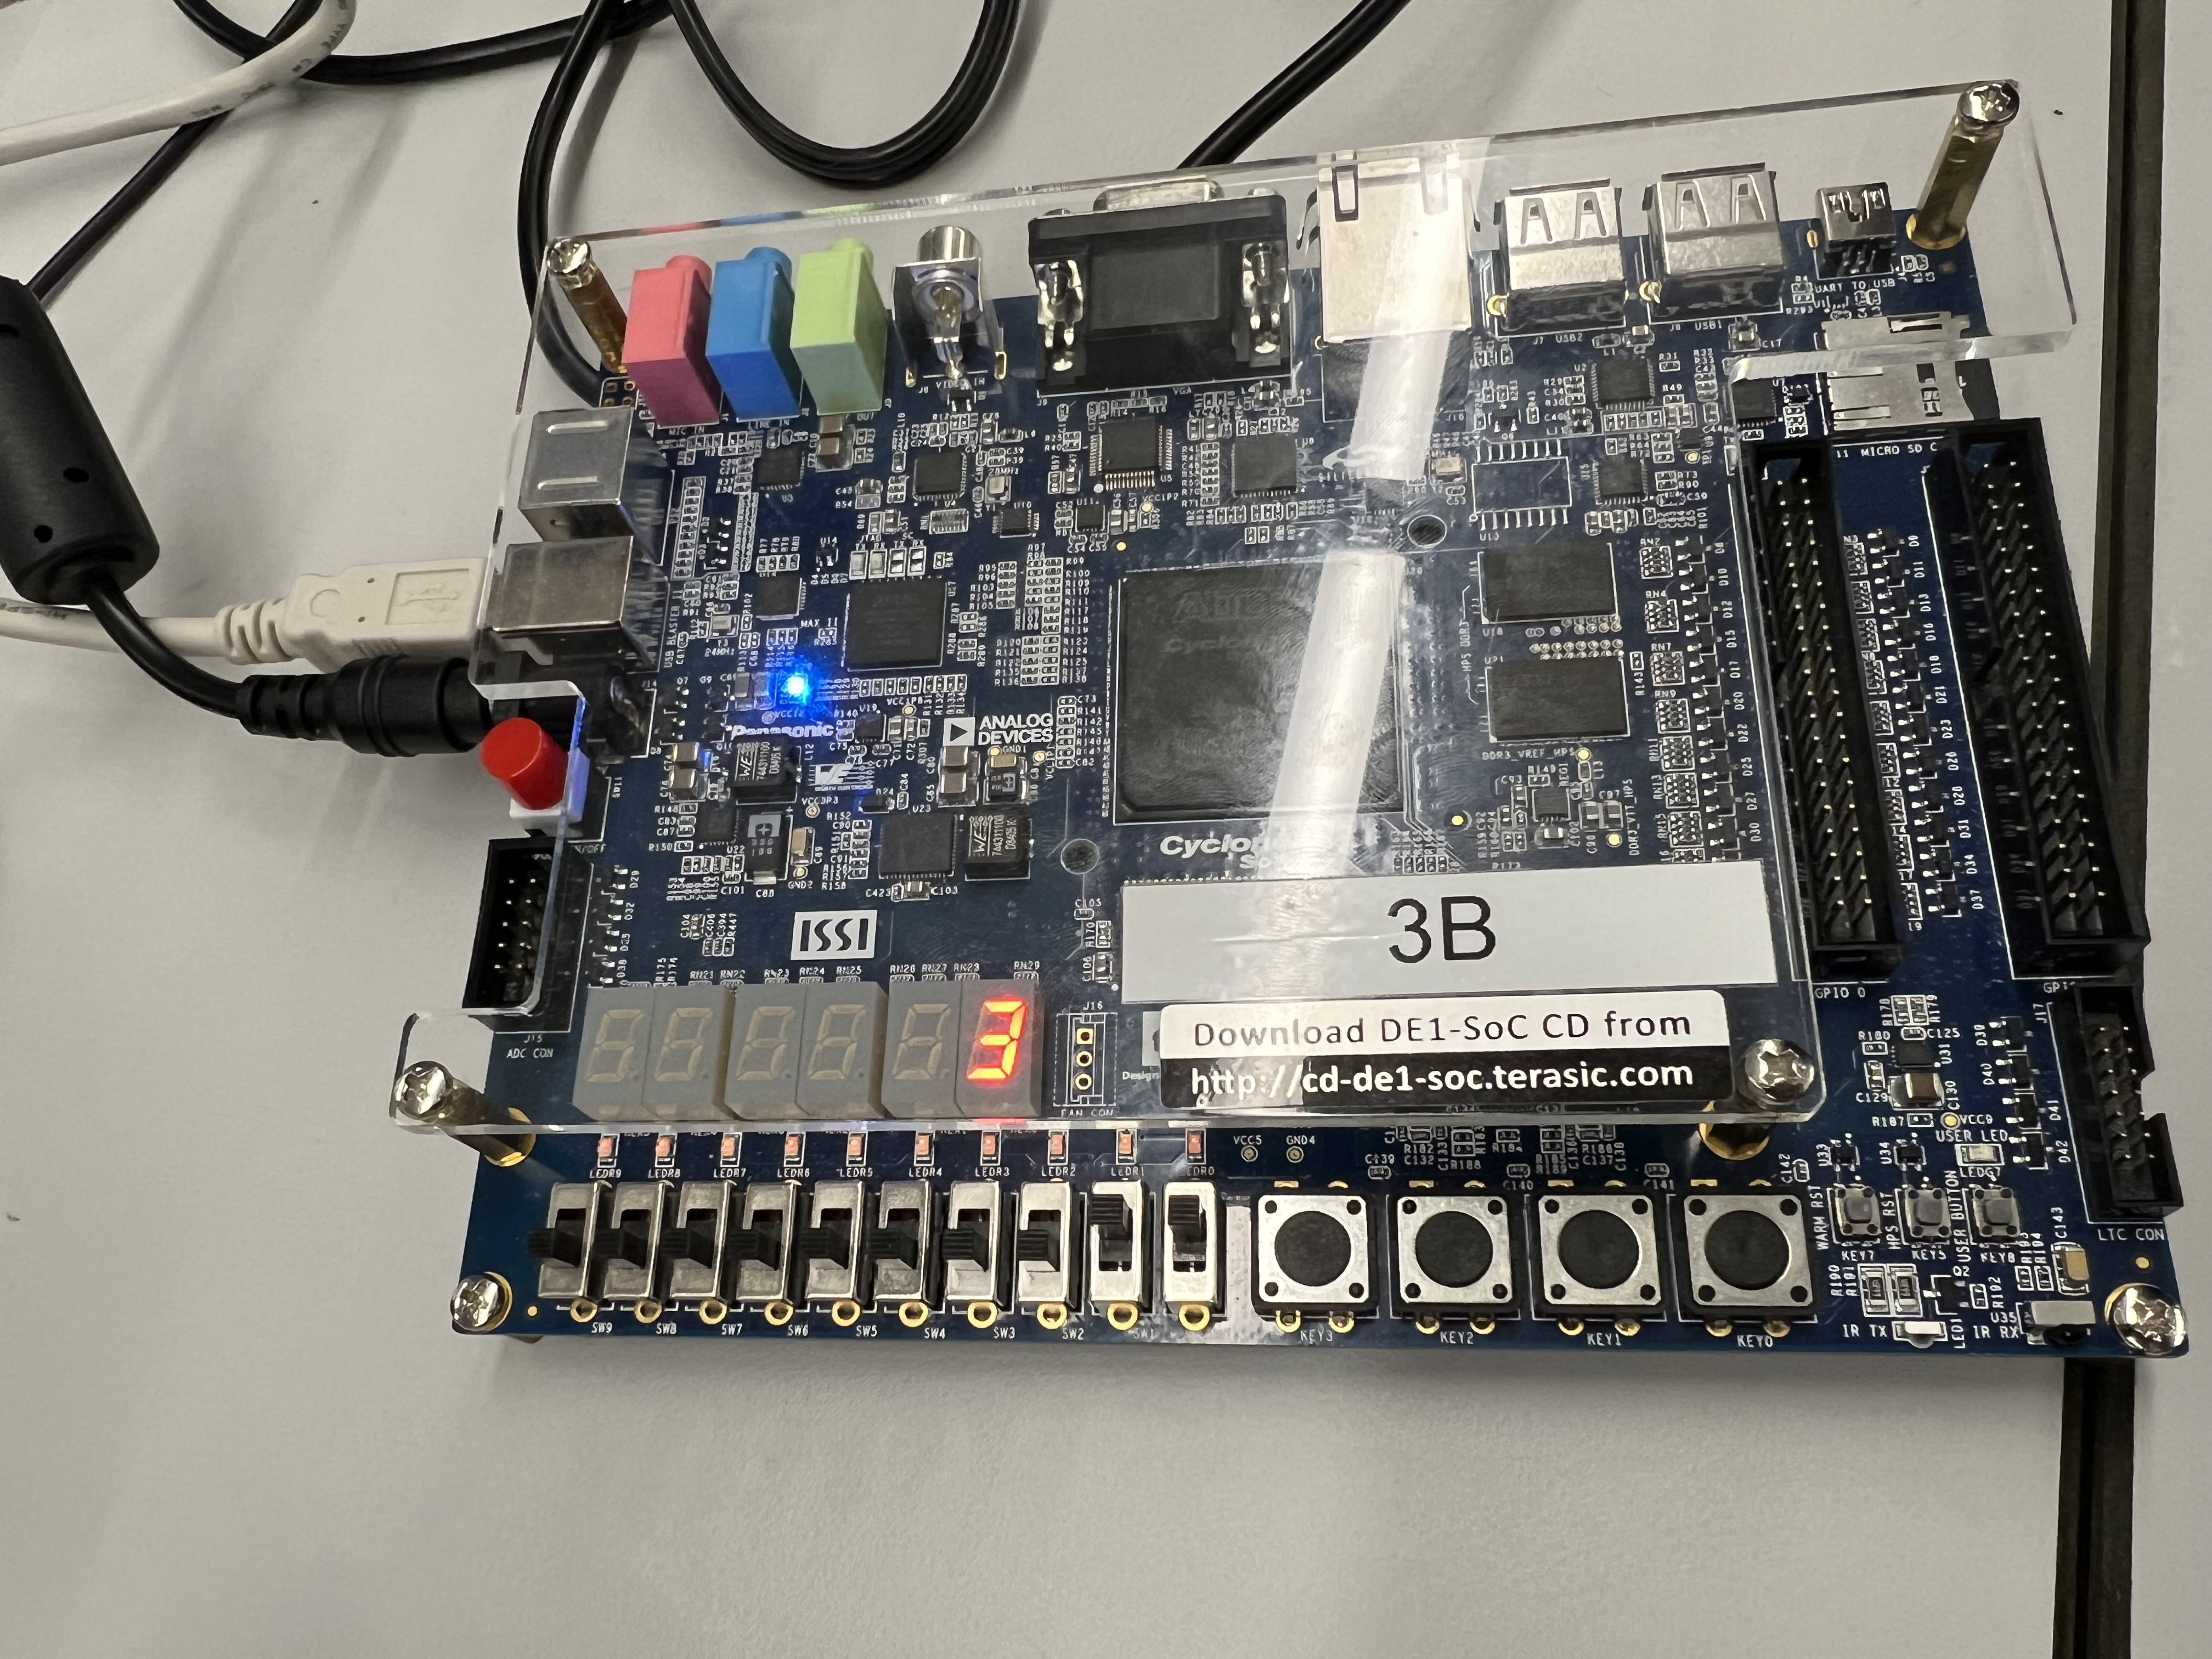
\includegraphics[width=.9\textwidth]{Figures/Disp_3.jpg}
  \caption{DE1-SoC Displaying 3 on HEX0 with input IN0 and IN1}
  \label{fig:6}
\end{figure}

\begin{figure}[H]
  \centering
  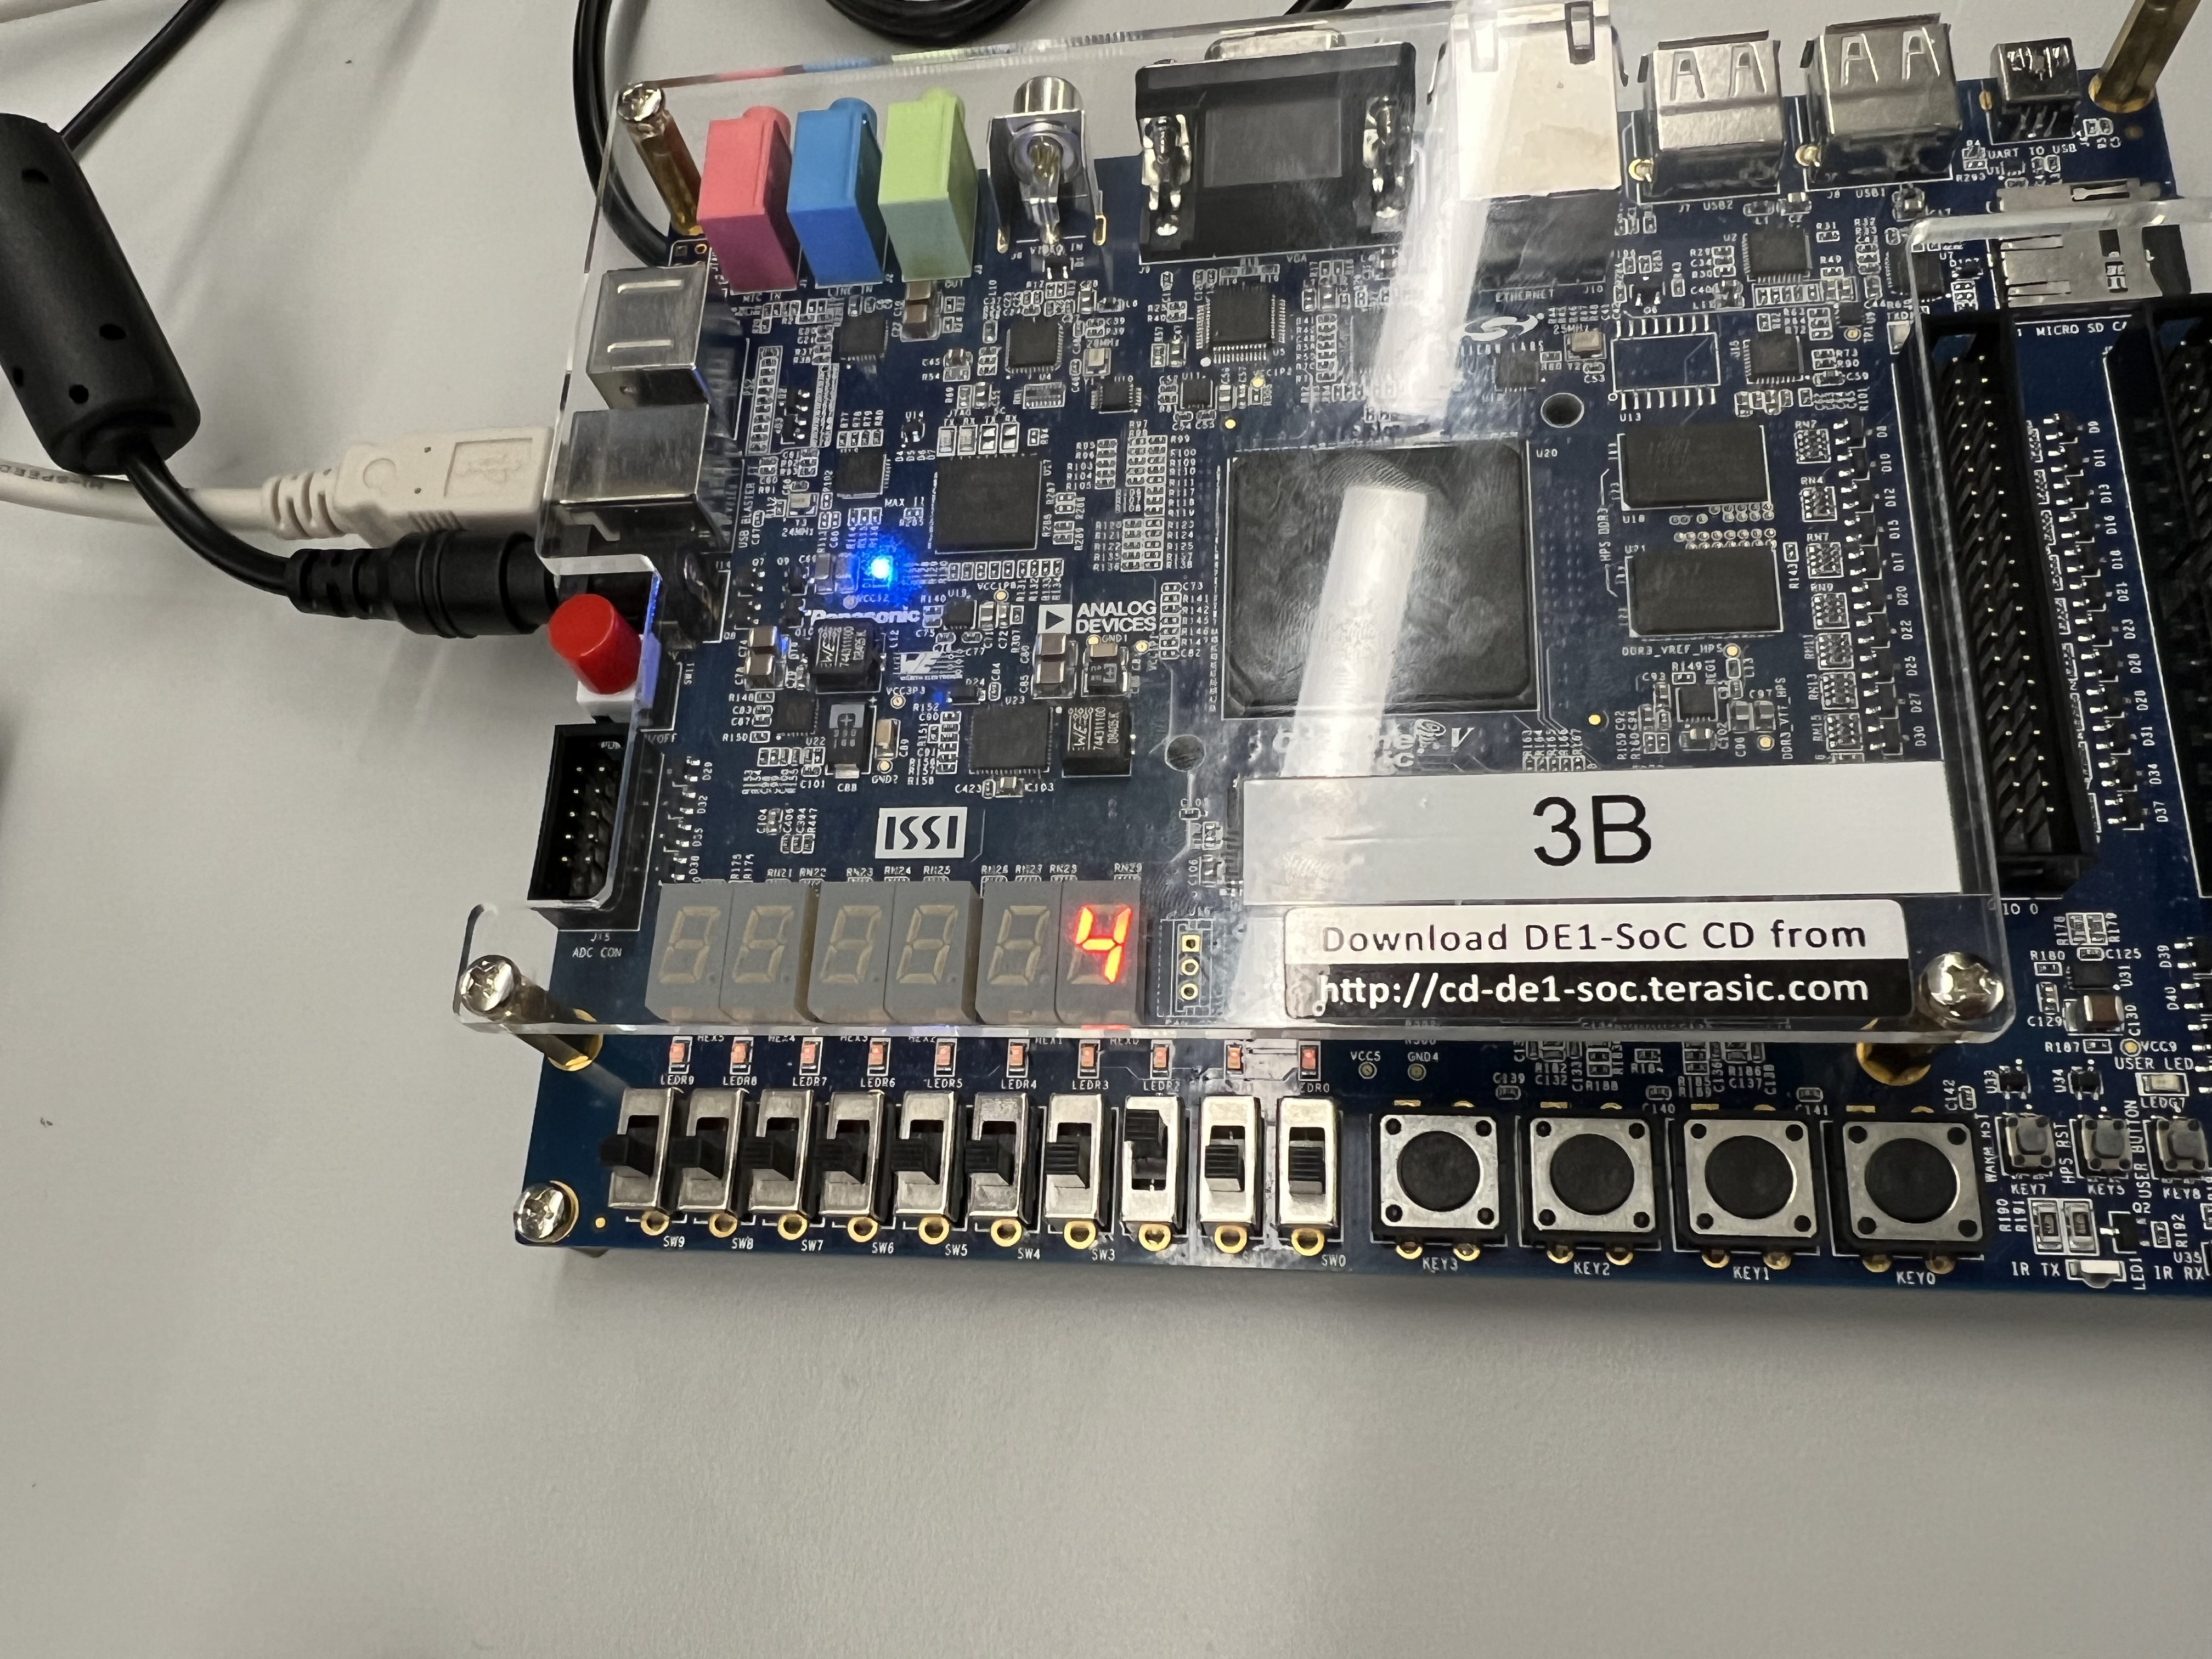
\includegraphics[width=.9\textwidth]{Figures/Disp_4.jpg}
  \caption{DE1-SoC Displaying 4 on HEX0 with input IN2}
  \label{fig:7}
\end{figure}

\begin{figure}[H]
  \centering
  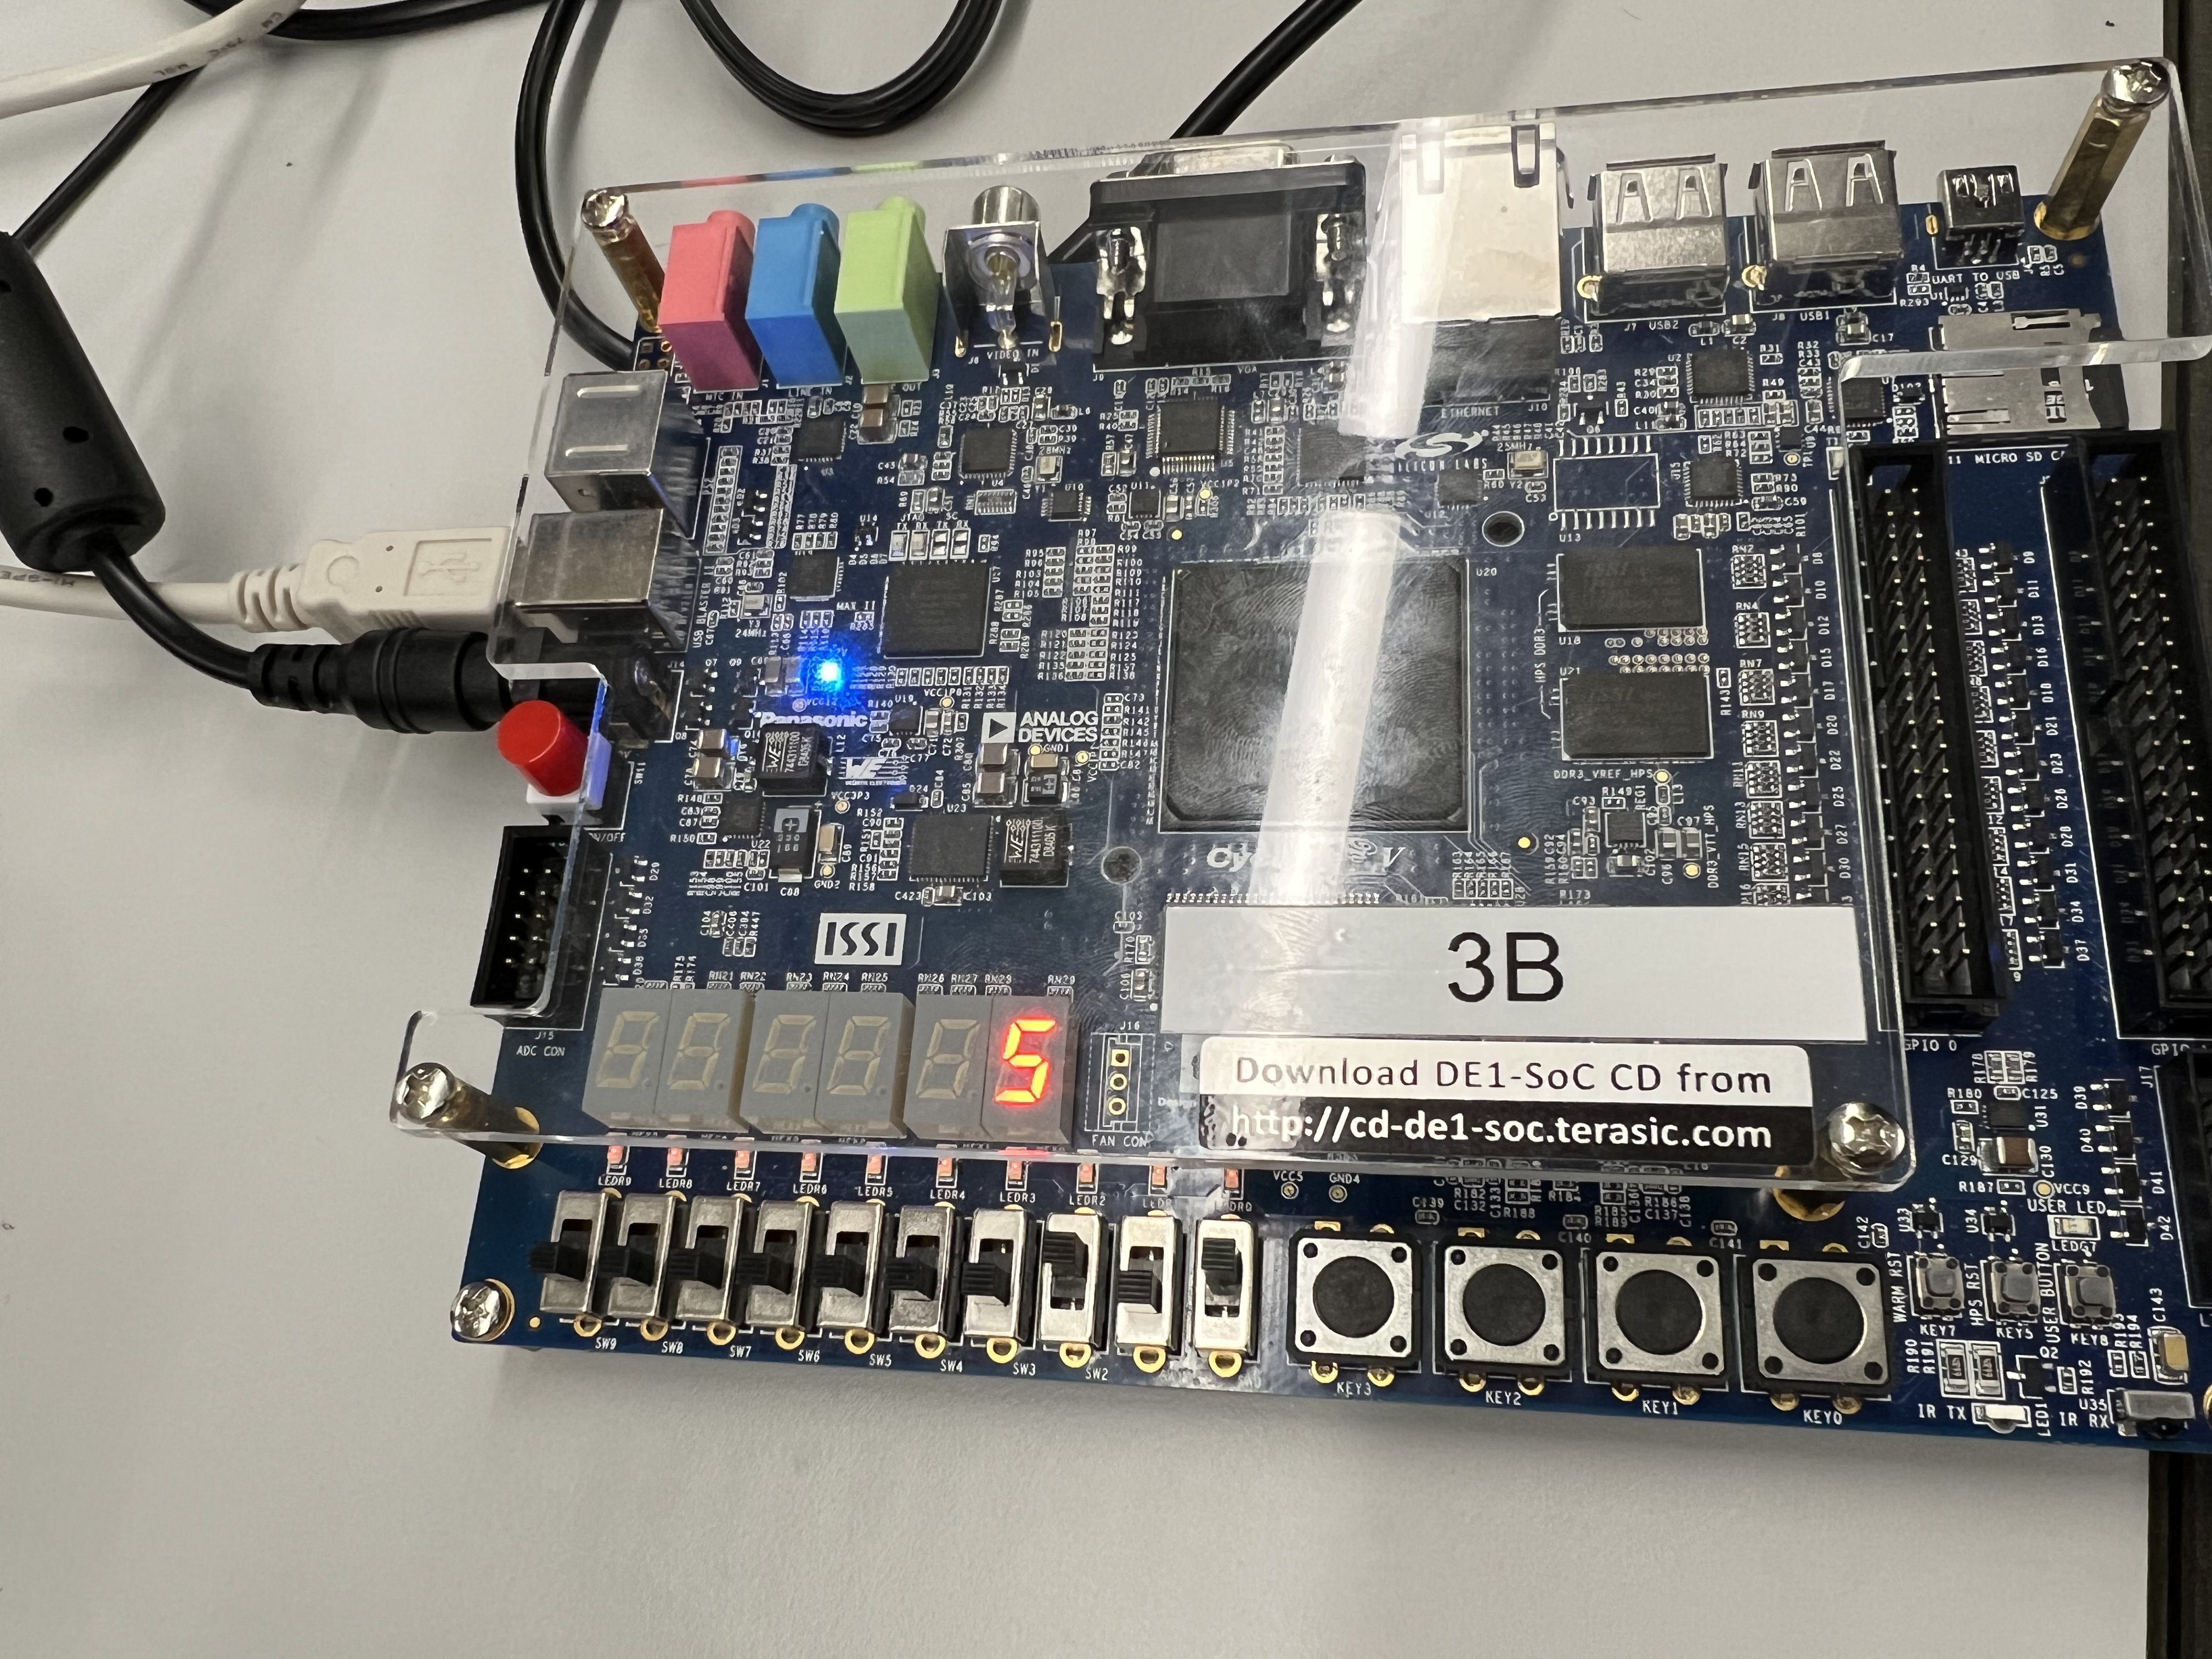
\includegraphics[width=.9\textwidth]{Figures/Disp_5.jpg}
  \caption{DE1-SoC Displaying 5 on HEX0 with input IN2 and IN0}
  \label{fig:8}
\end{figure}

\begin{figure}[H]
  \centering
  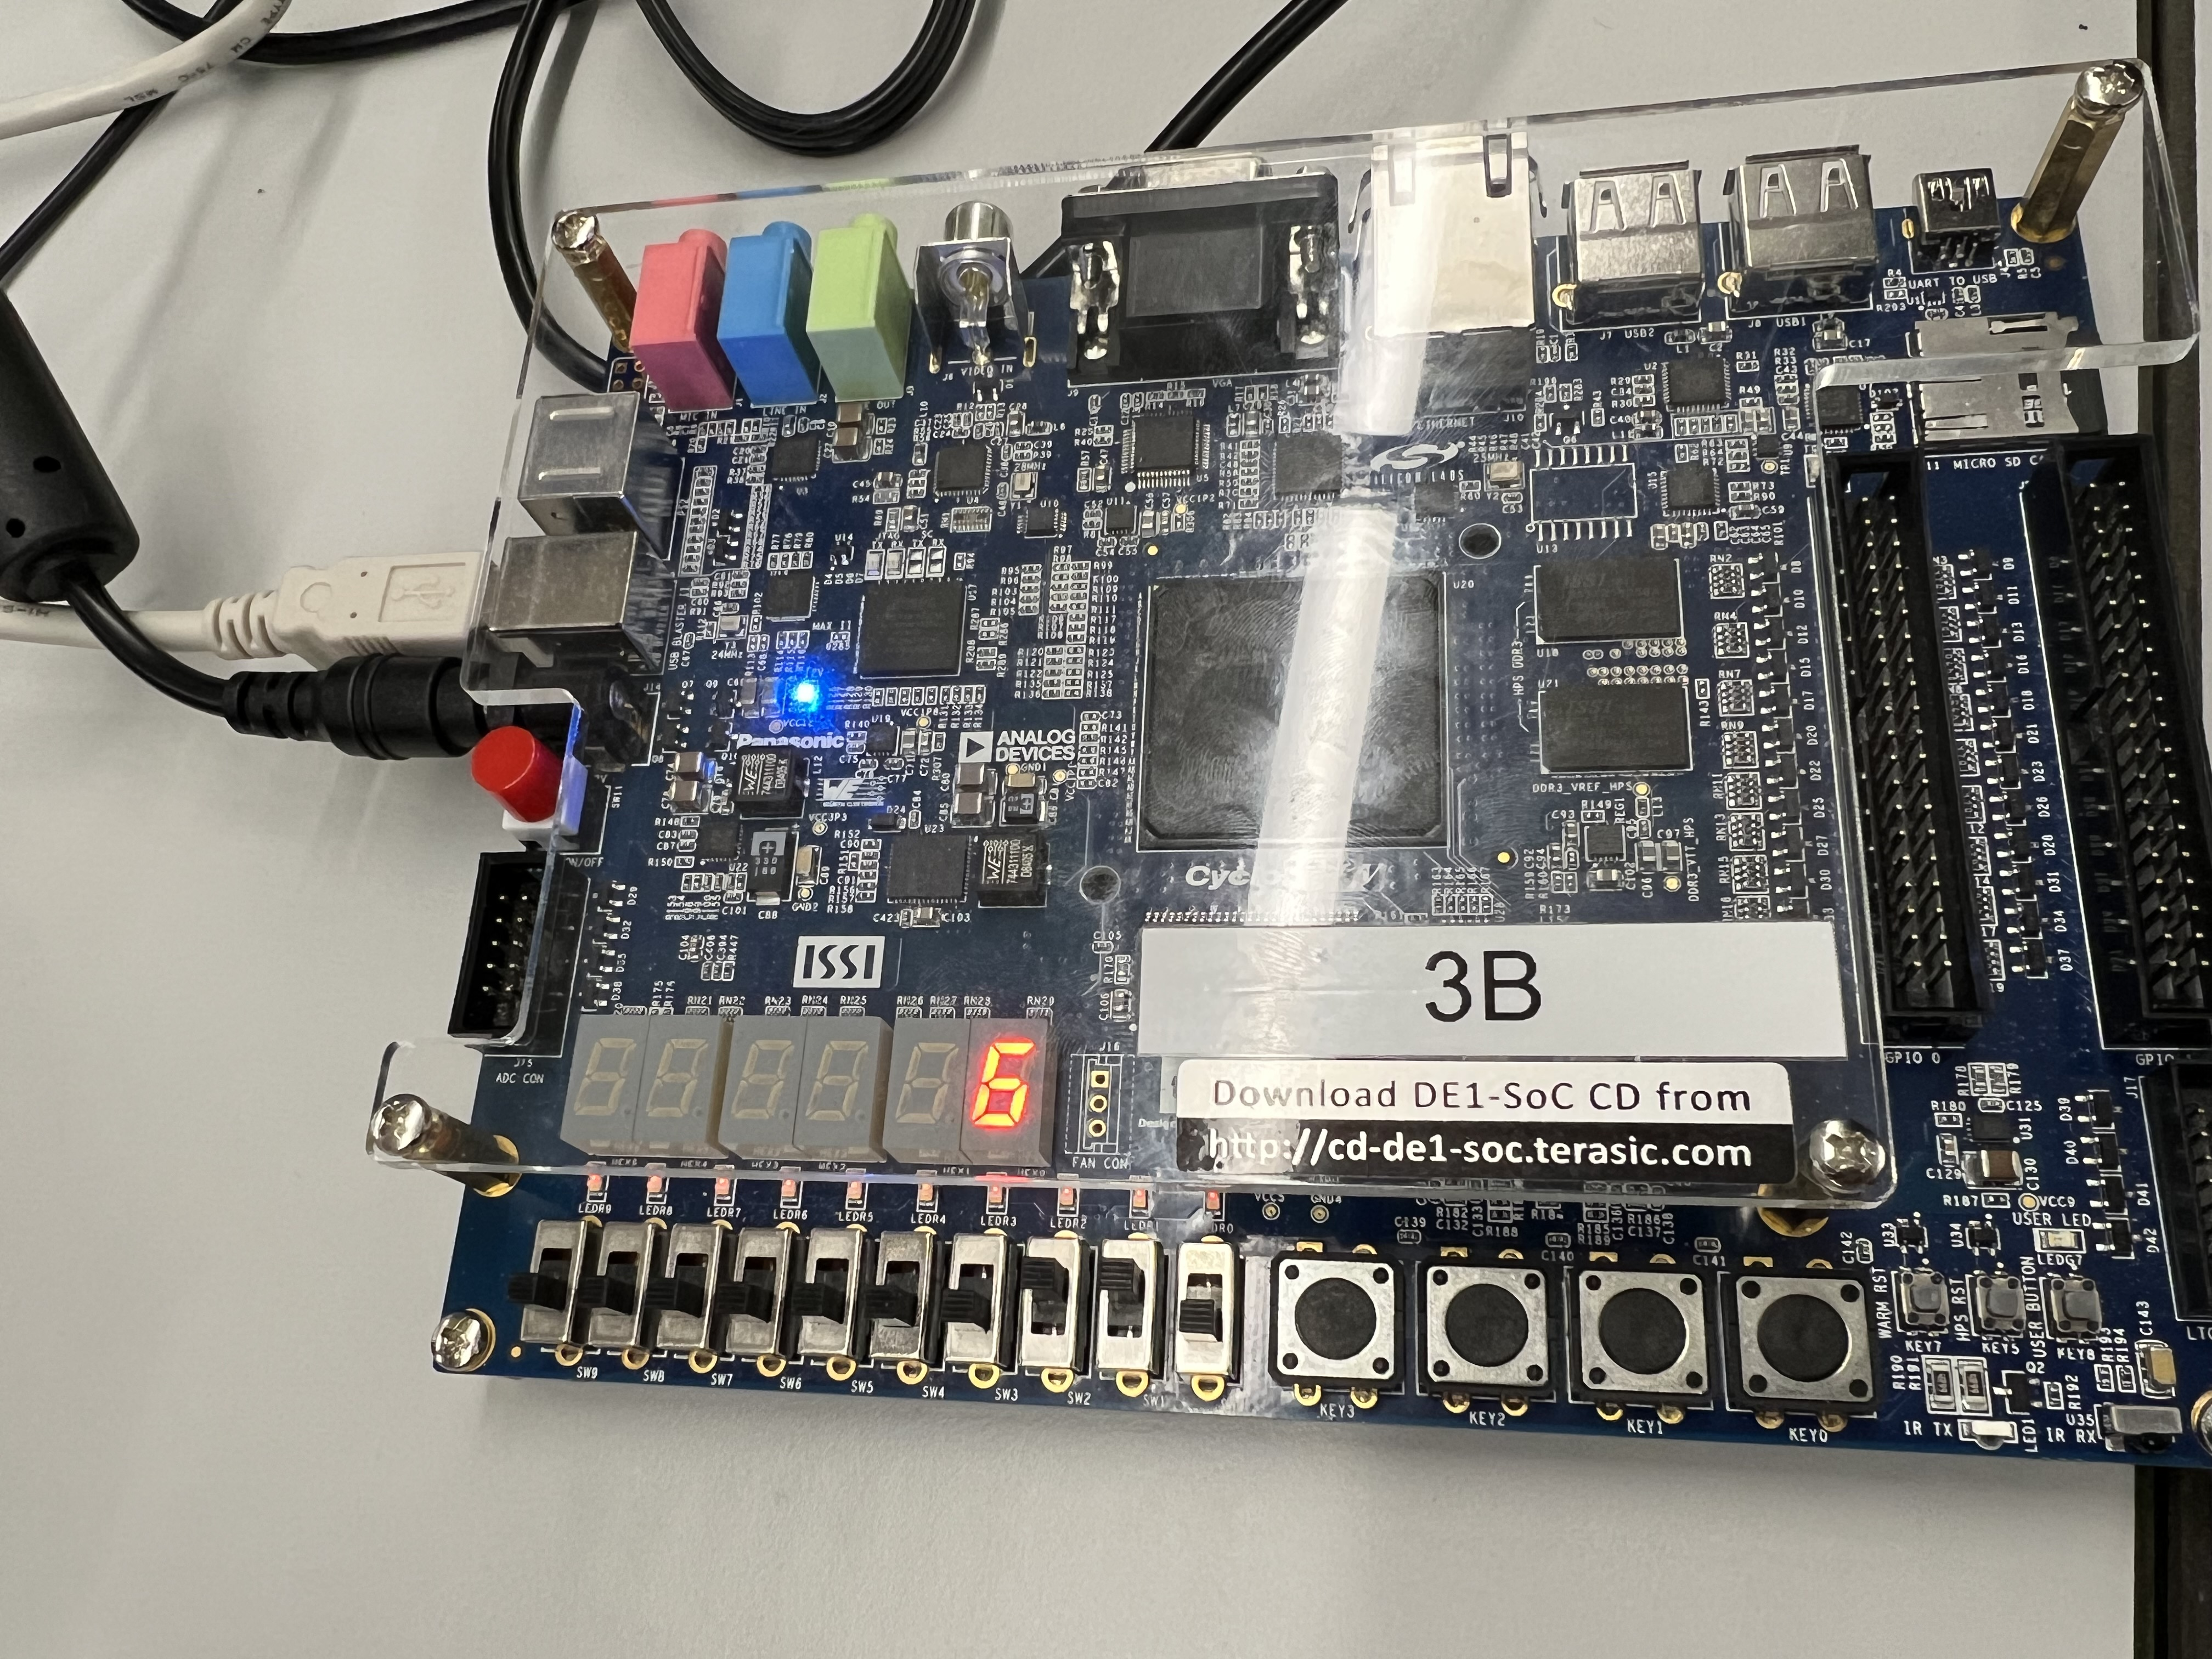
\includegraphics[width=.9\textwidth]{Figures/Disp_6.jpg}
  \caption{DE1-SoC Displaying 6 on HEX0 with input IN1 and IN2}
  \label{fig:9}
\end{figure}

\begin{figure}[H]
  \centering
  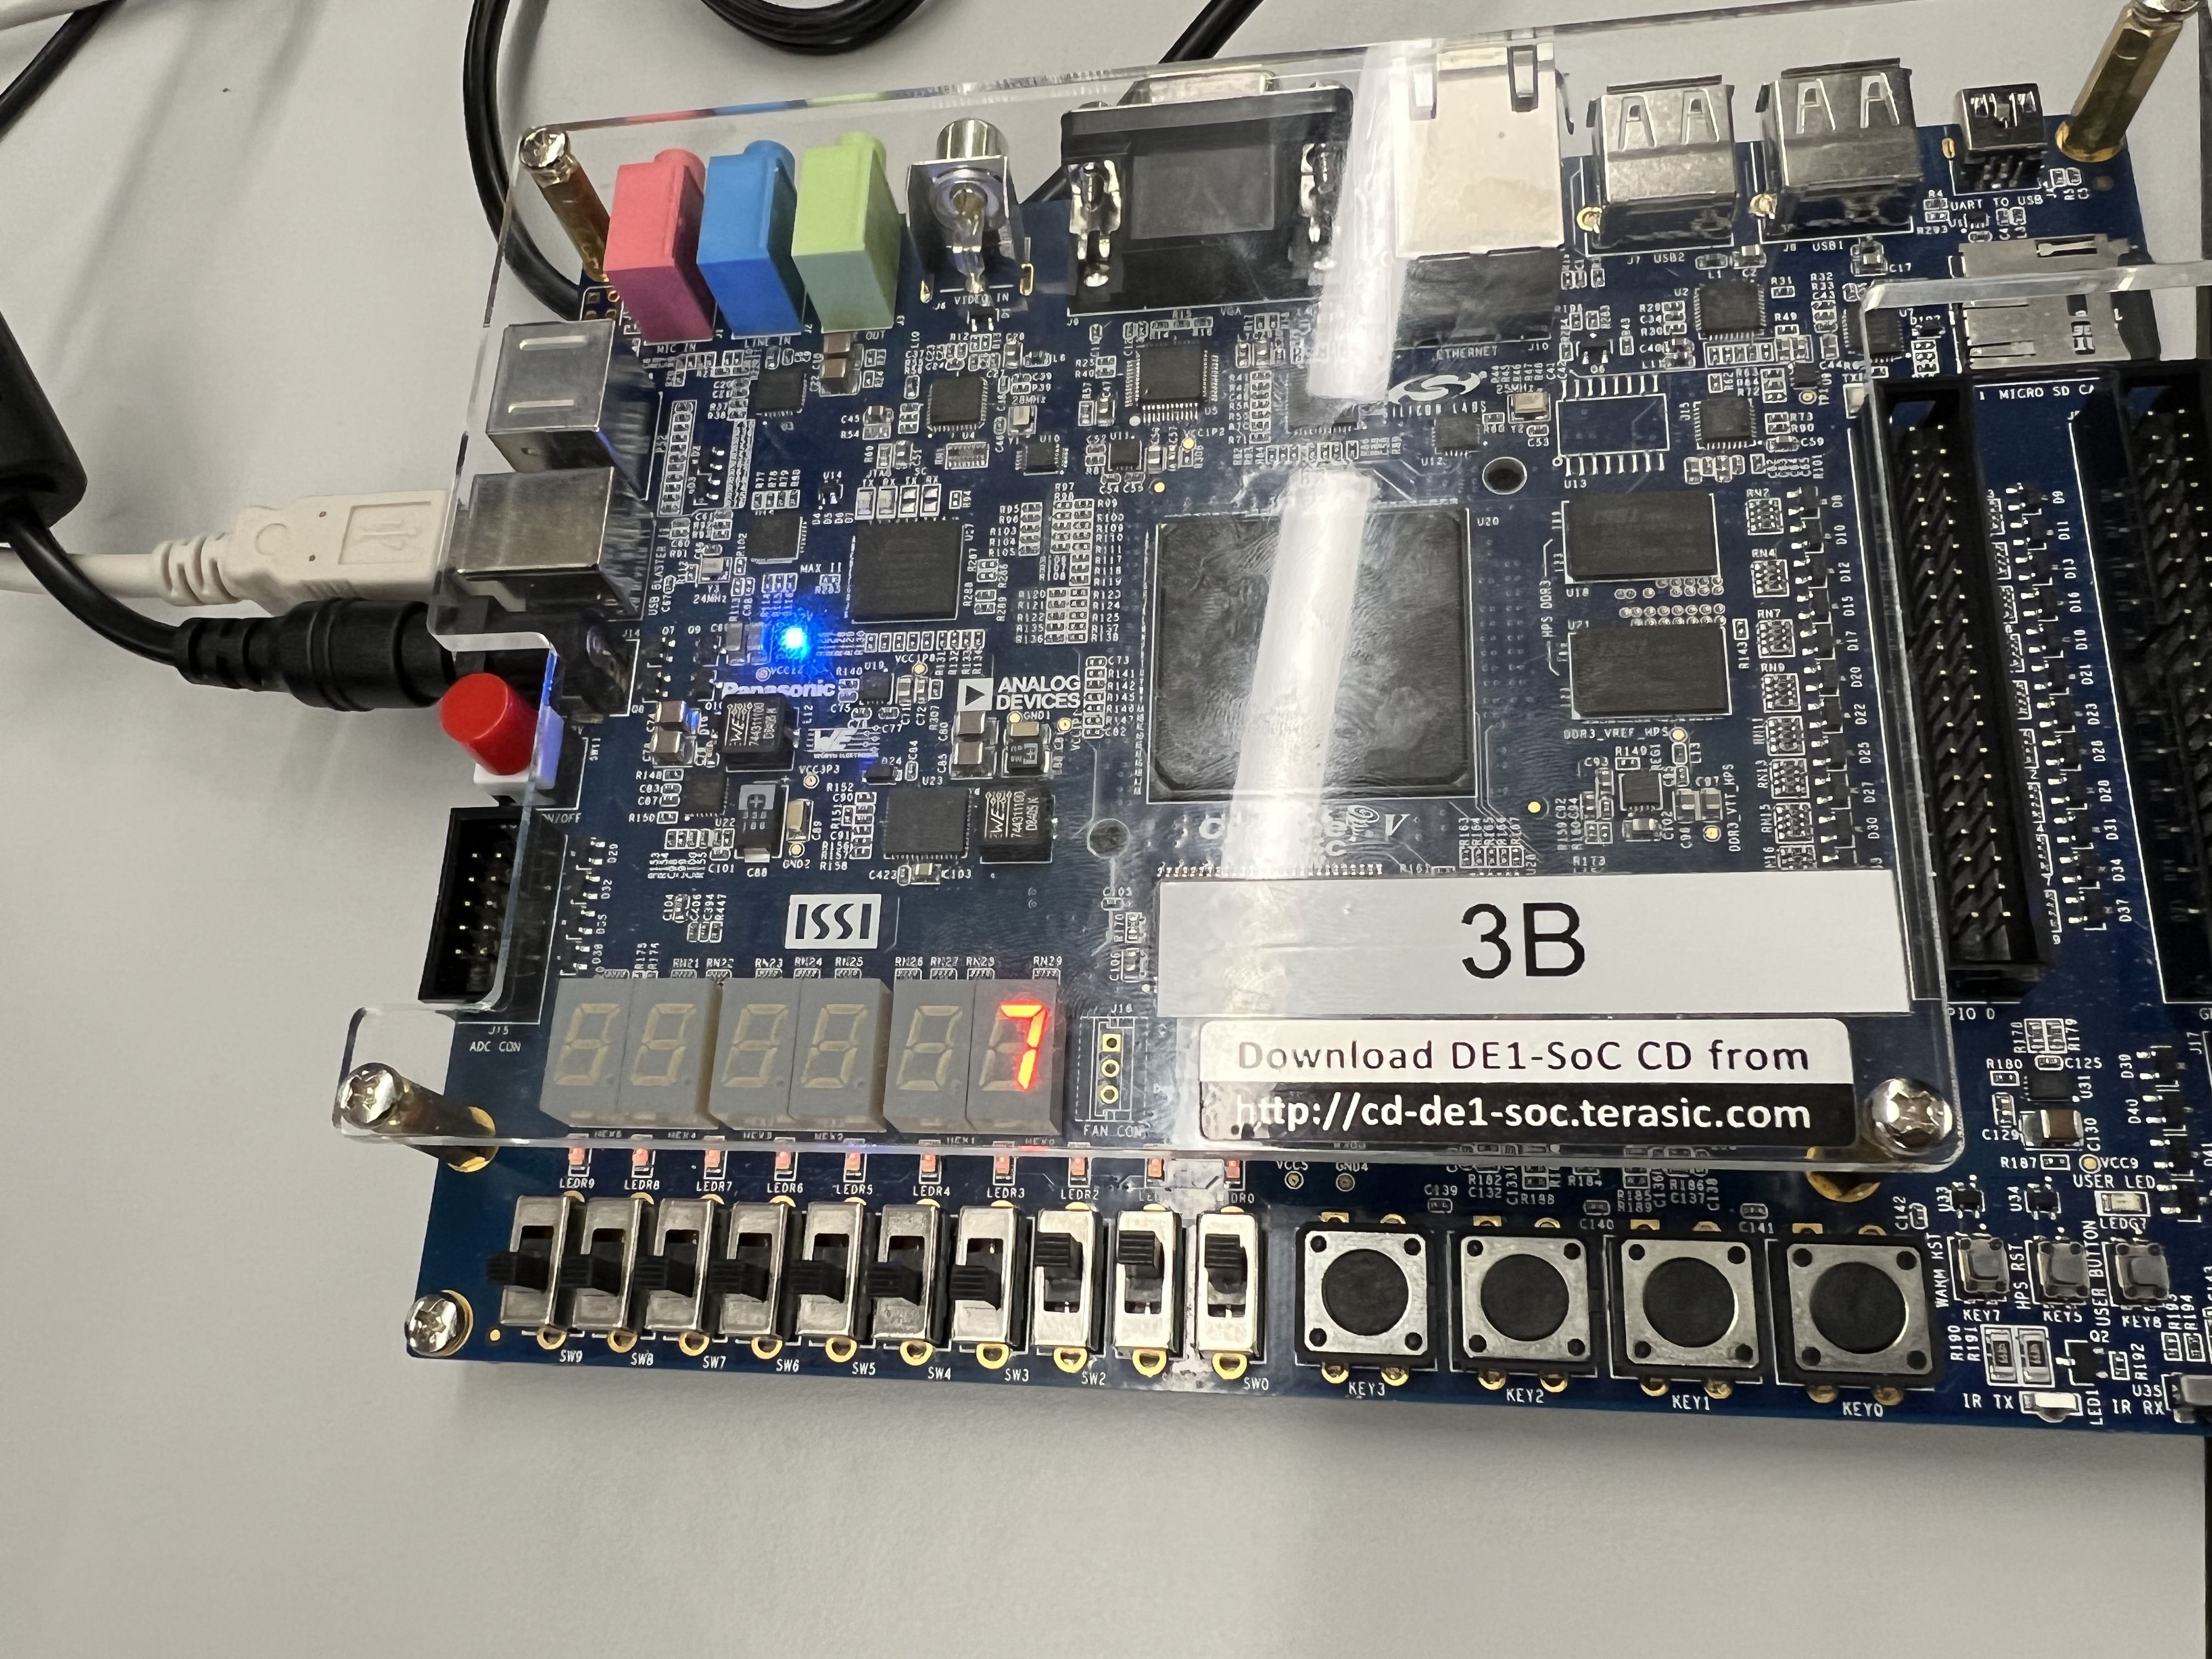
\includegraphics[width=.9\textwidth]{Figures/Disp_7.jpg}
  \caption{DE1-SoC Displaying 7 on HEX0 with input IN0, IN1, and IN2}
  \label{fig:10}
\end{figure}

\begin{figure}[H]
  \centering
  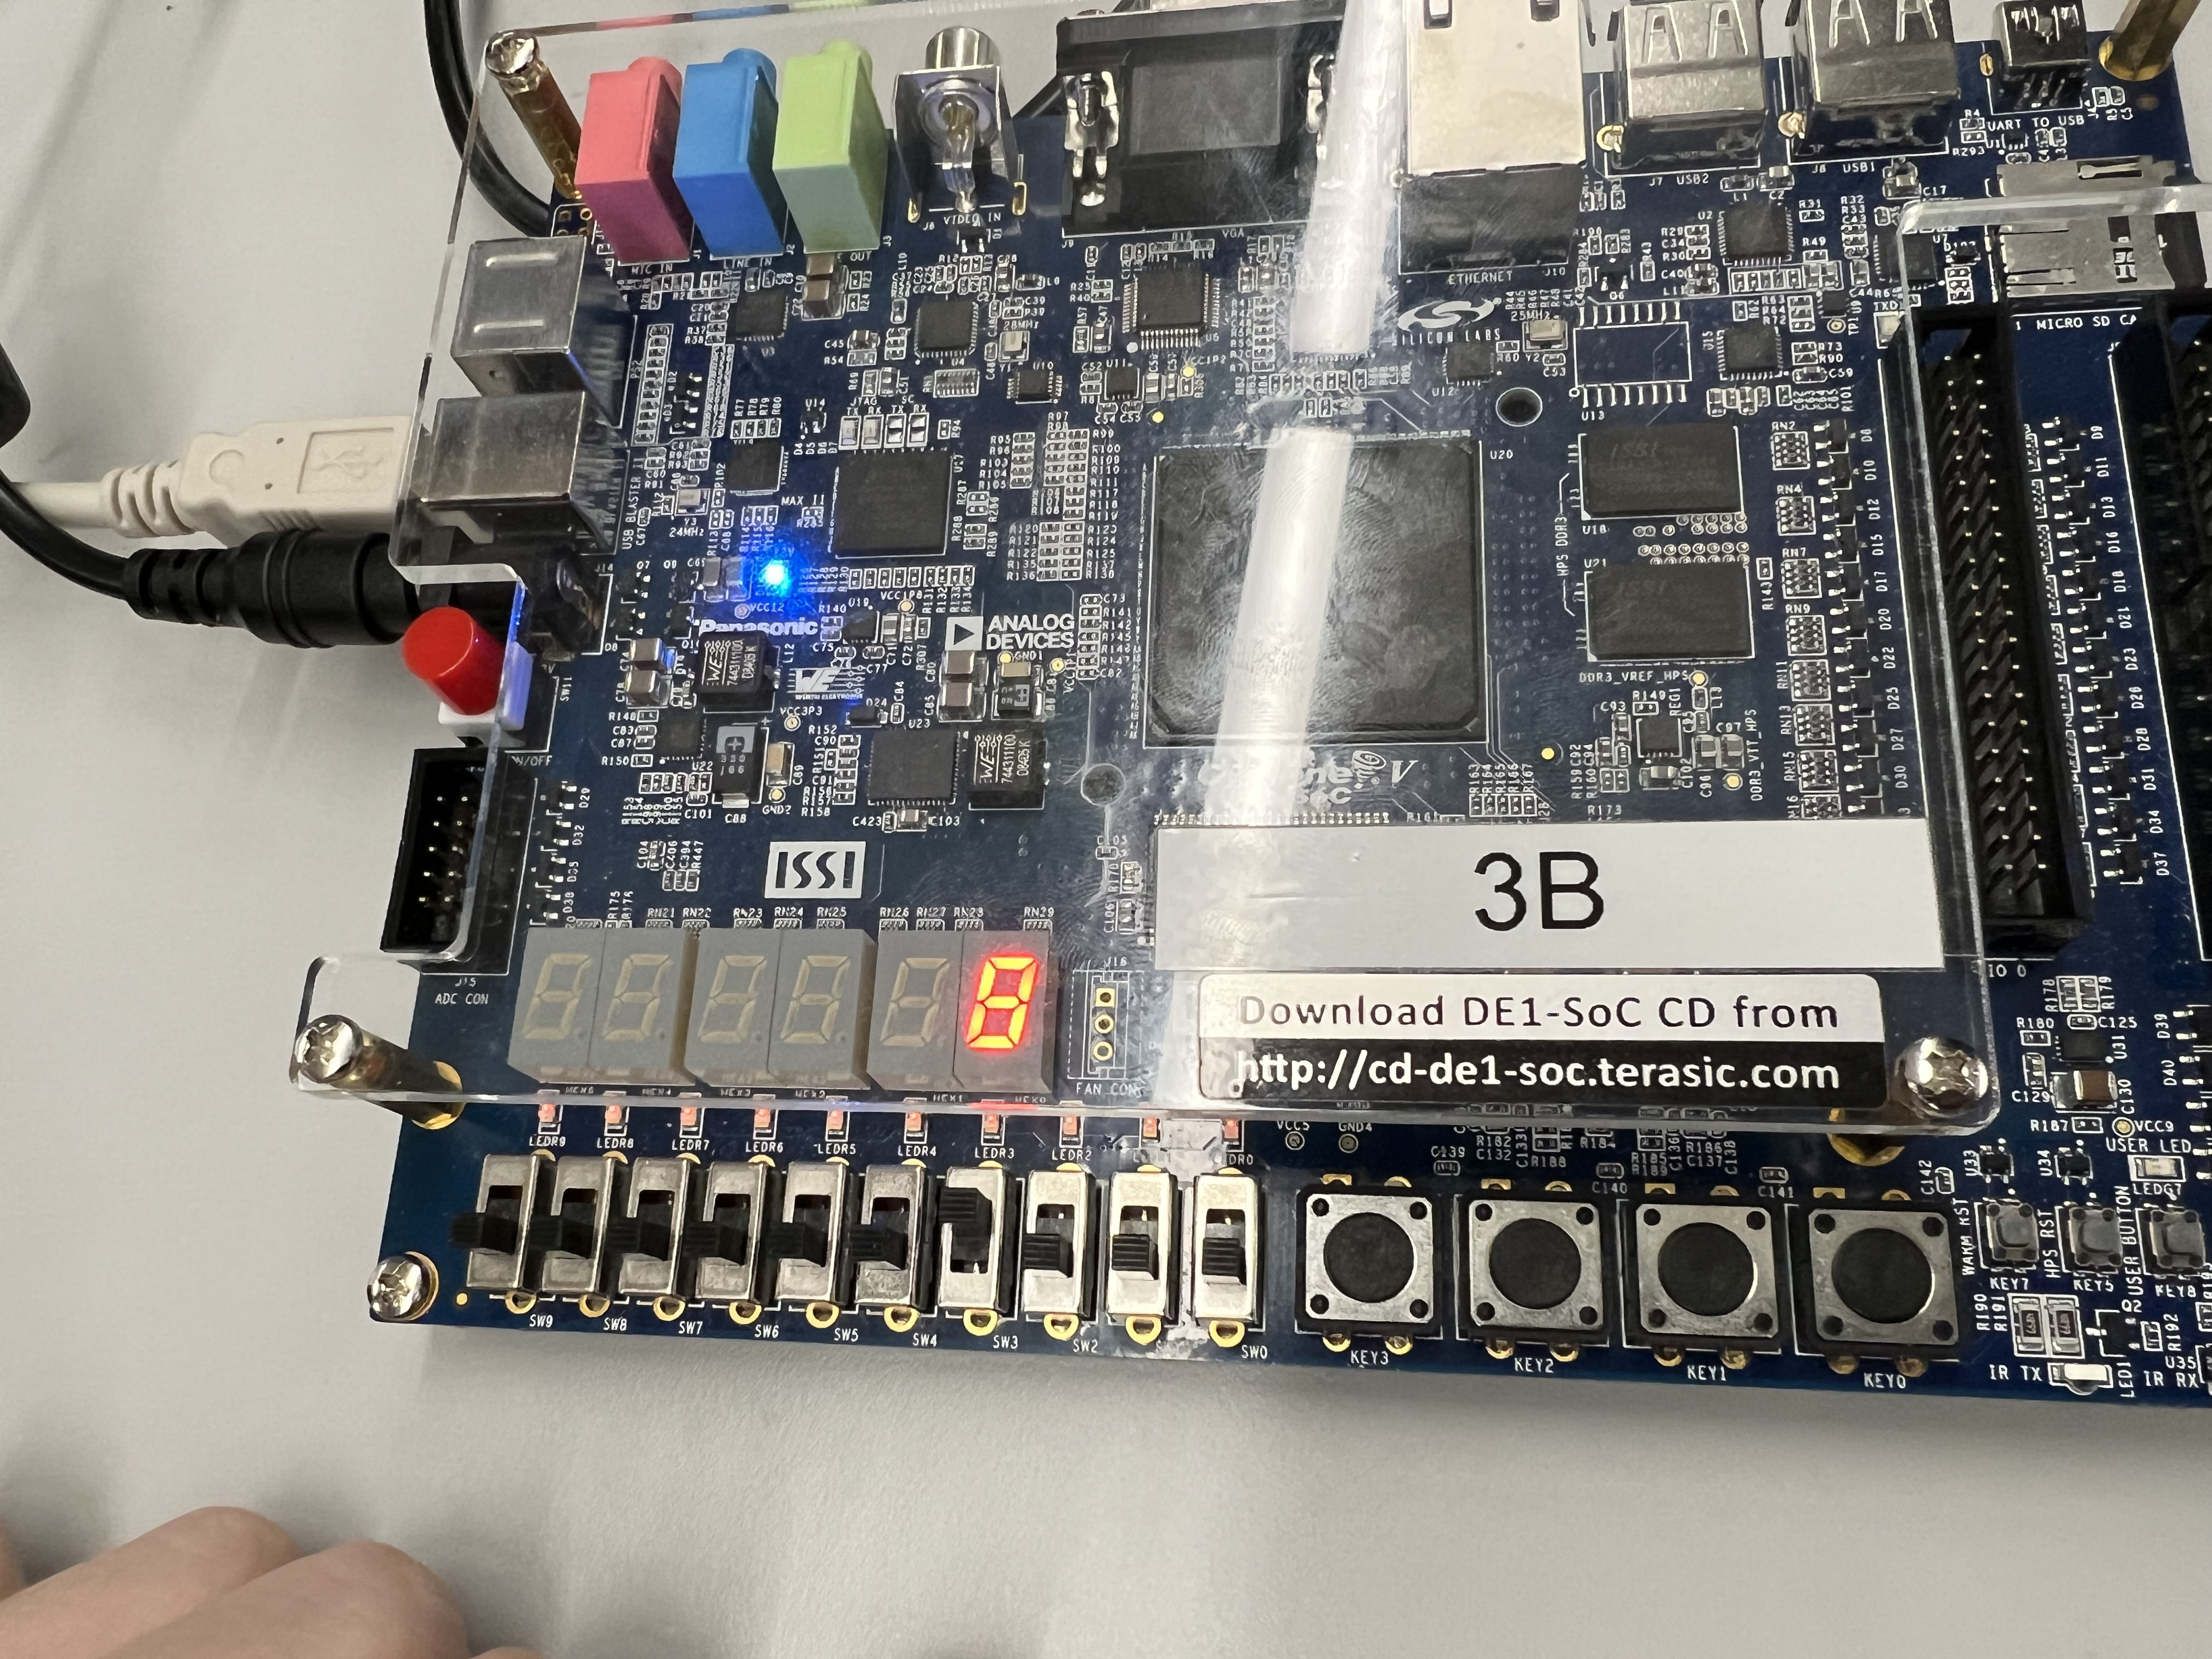
\includegraphics[width=.9\textwidth]{Figures/Disp_8.jpg}
  \caption{DE1-SoC Displaying 8 on HEX0 with input IN3}
  \label{fig:11}
\end{figure}

\begin{figure}[H]
  \centering
  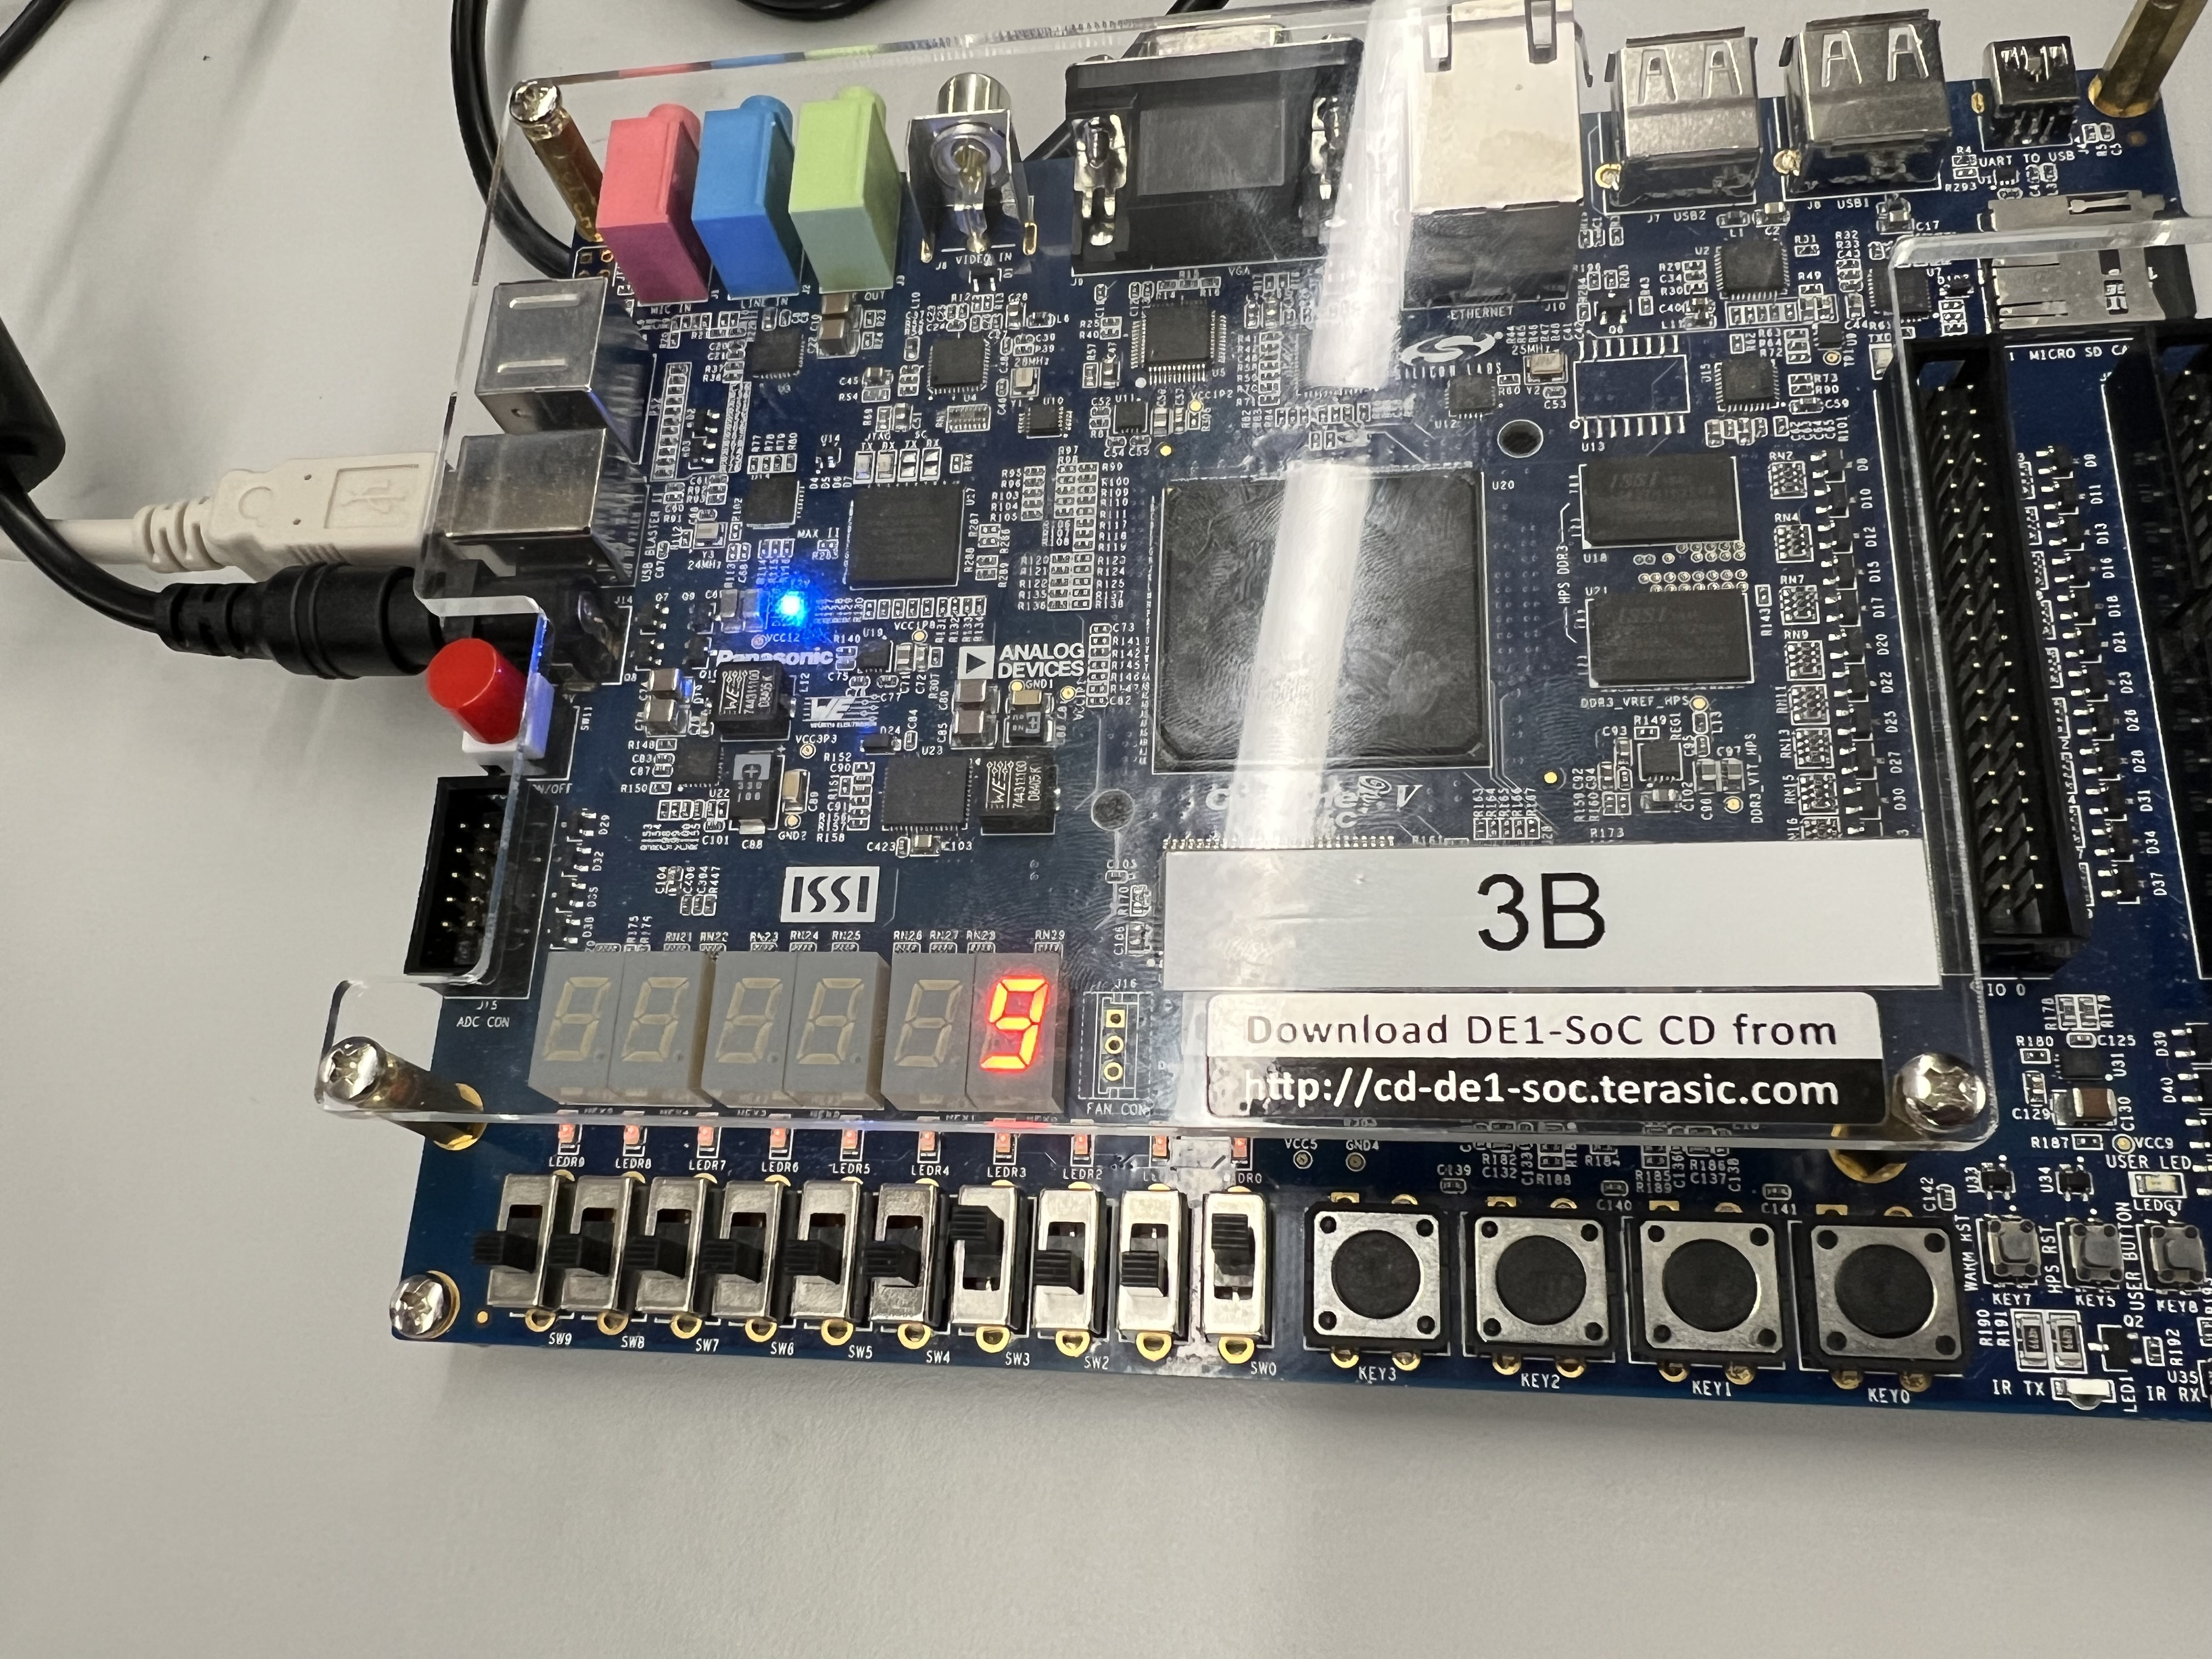
\includegraphics[width=.9\textwidth]{Figures/Disp_9.jpg}
  \caption{DE1-SoC Displaying 9 on HEX0 with input IN0 and IN3}
  \label{fig:12}
\end{figure}

\hspace{.5 in} All displayed numbers with corresponding inputs on the DE1-SoC board matched the expected outputs from the truth table. 

\subsection{Assignment 3}

\hspace{.5 in} In Assignment 3, the goal was to have the ability for the display to be off, meaning all the segments are off, when not in use. To do this, an enable input, that acted as an on/off switch, was added into the circuit design, as shown in Figure \ref{fig:13} below.

\begin{figure}[H]
  \centering
  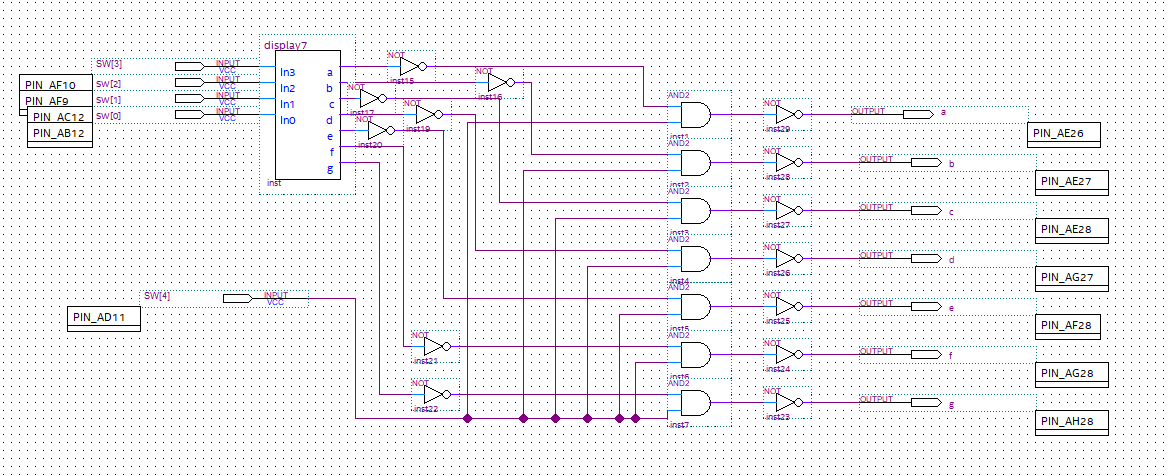
\includegraphics[width=.9\textwidth]{Figures/Design_en.png}
  \caption{Compressed digital display block with additional input and logic to act as an enable switch}
  \label{fig:13}
\end{figure}

\hspace{.5 in} As can be seen in Figure \ref{fig:13}, in order to add the enable input, the digital display design created in Assignment 1 was packed into a logic block called display7. The output of display7, which are the segments that are to be turned on, were inverted with NOT gates and inputted into separate AND gates with the enable input. Thus, all the on segments with an output of 0 are inverted to 1 and all off segments with an output of 1 were inverted to 0. In the case of the enable input being 0, the on segments (now 1’s) going into the AND gate with the enable input of 0, will output all 0. Additionally, all the off segments (now 0’s) go into the AND gate with the enable input of 0, which will output all 0. However, 0 designates that a segment is on, so additional NOT gates were added after the AND gates to invert all 0’s to 1’s. To adequately test this circuit, a simulation was run with the Waveform Simulation software. The results of the simulation are shown in Figure \ref{fig:14}.

\begin{figure}[H]
  \centering
  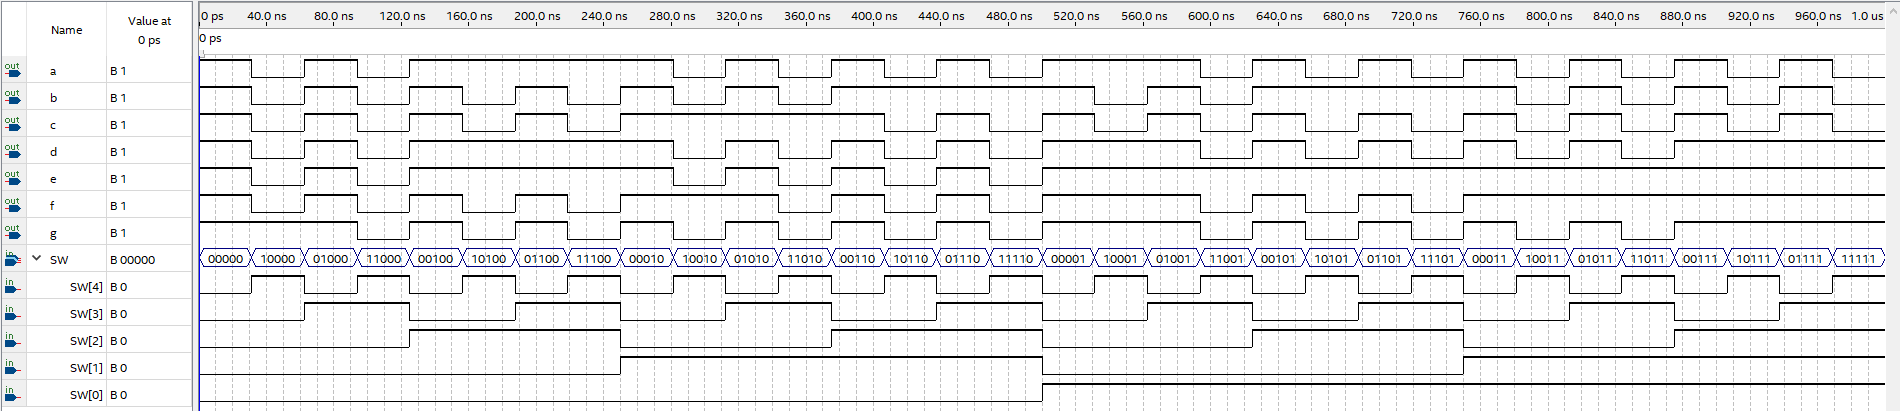
\includegraphics[width=.9\textwidth]{Figures/Sim_en.png}
  \caption{Waveform Simulation Results With an Enable Input (SW[4])}
  \label{fig:14}
\end{figure}

From the simulation results, it can be seen that when SW[4] (the enable input) is 0 then all the Segment outputs are 1, which in our case means they are off. Then when SW[4] is 1, the segment outputs correspond to the number that is supposed to be displayed. 

\subsection{Assignment 4}

In Assignment 4, the goal was to display a digit on multiple 7-Segment displays if the display is enabled. To display a digit on multiple 7-Segment displays if the display is enabled, the circuit design from Assignment 3 was packed into a logic block called display7\_en. Six of the display7\_en logic blocks, one for each available 7-Segment display on the DE1-SoC board were used to create the circuit design shown in Figure \ref{fig:15} below. 

\begin{figure}[H]
  \centering
  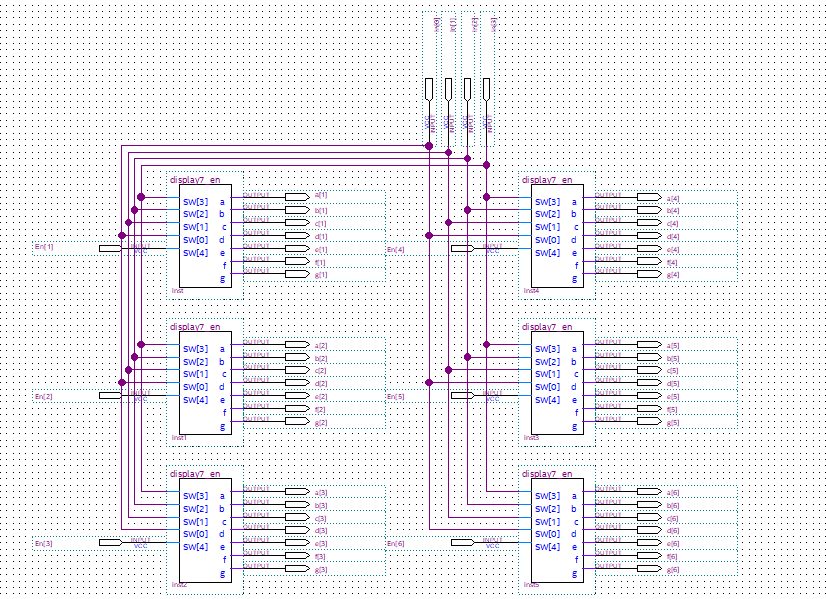
\includegraphics[width=.9\textwidth]{Figures/display_control.png}
  \caption{Circuit design for displaying a digit on multiple 7-Segment displays if the display is enabled}
  \label{fig:15}
\end{figure}

For the inputs, the digits 0-9 being displayed were represented by the first four switches SW[0], SW[1], SW[2], and SW[3]. As for enabling the displays, SW[4], SW[5], SW[6], SW[7], SW[8], and SW[9] were used. Then, for the outputs, they were assigned to each of the six displayed HEX0, HEX1, HEX2, HEX3, HEX4, and HEX5. Once the design was completed with the correct assignments, it was uploaded to the DE1-SoC board for testing. The switches were changed around to verify the correct behavior and output on the displays given different inputs. Images of the Board with switches in different positions are shown in Figures \ref{fig:16}-\ref{fig:19} below. 

\begin{figure}[H]
  \centering
  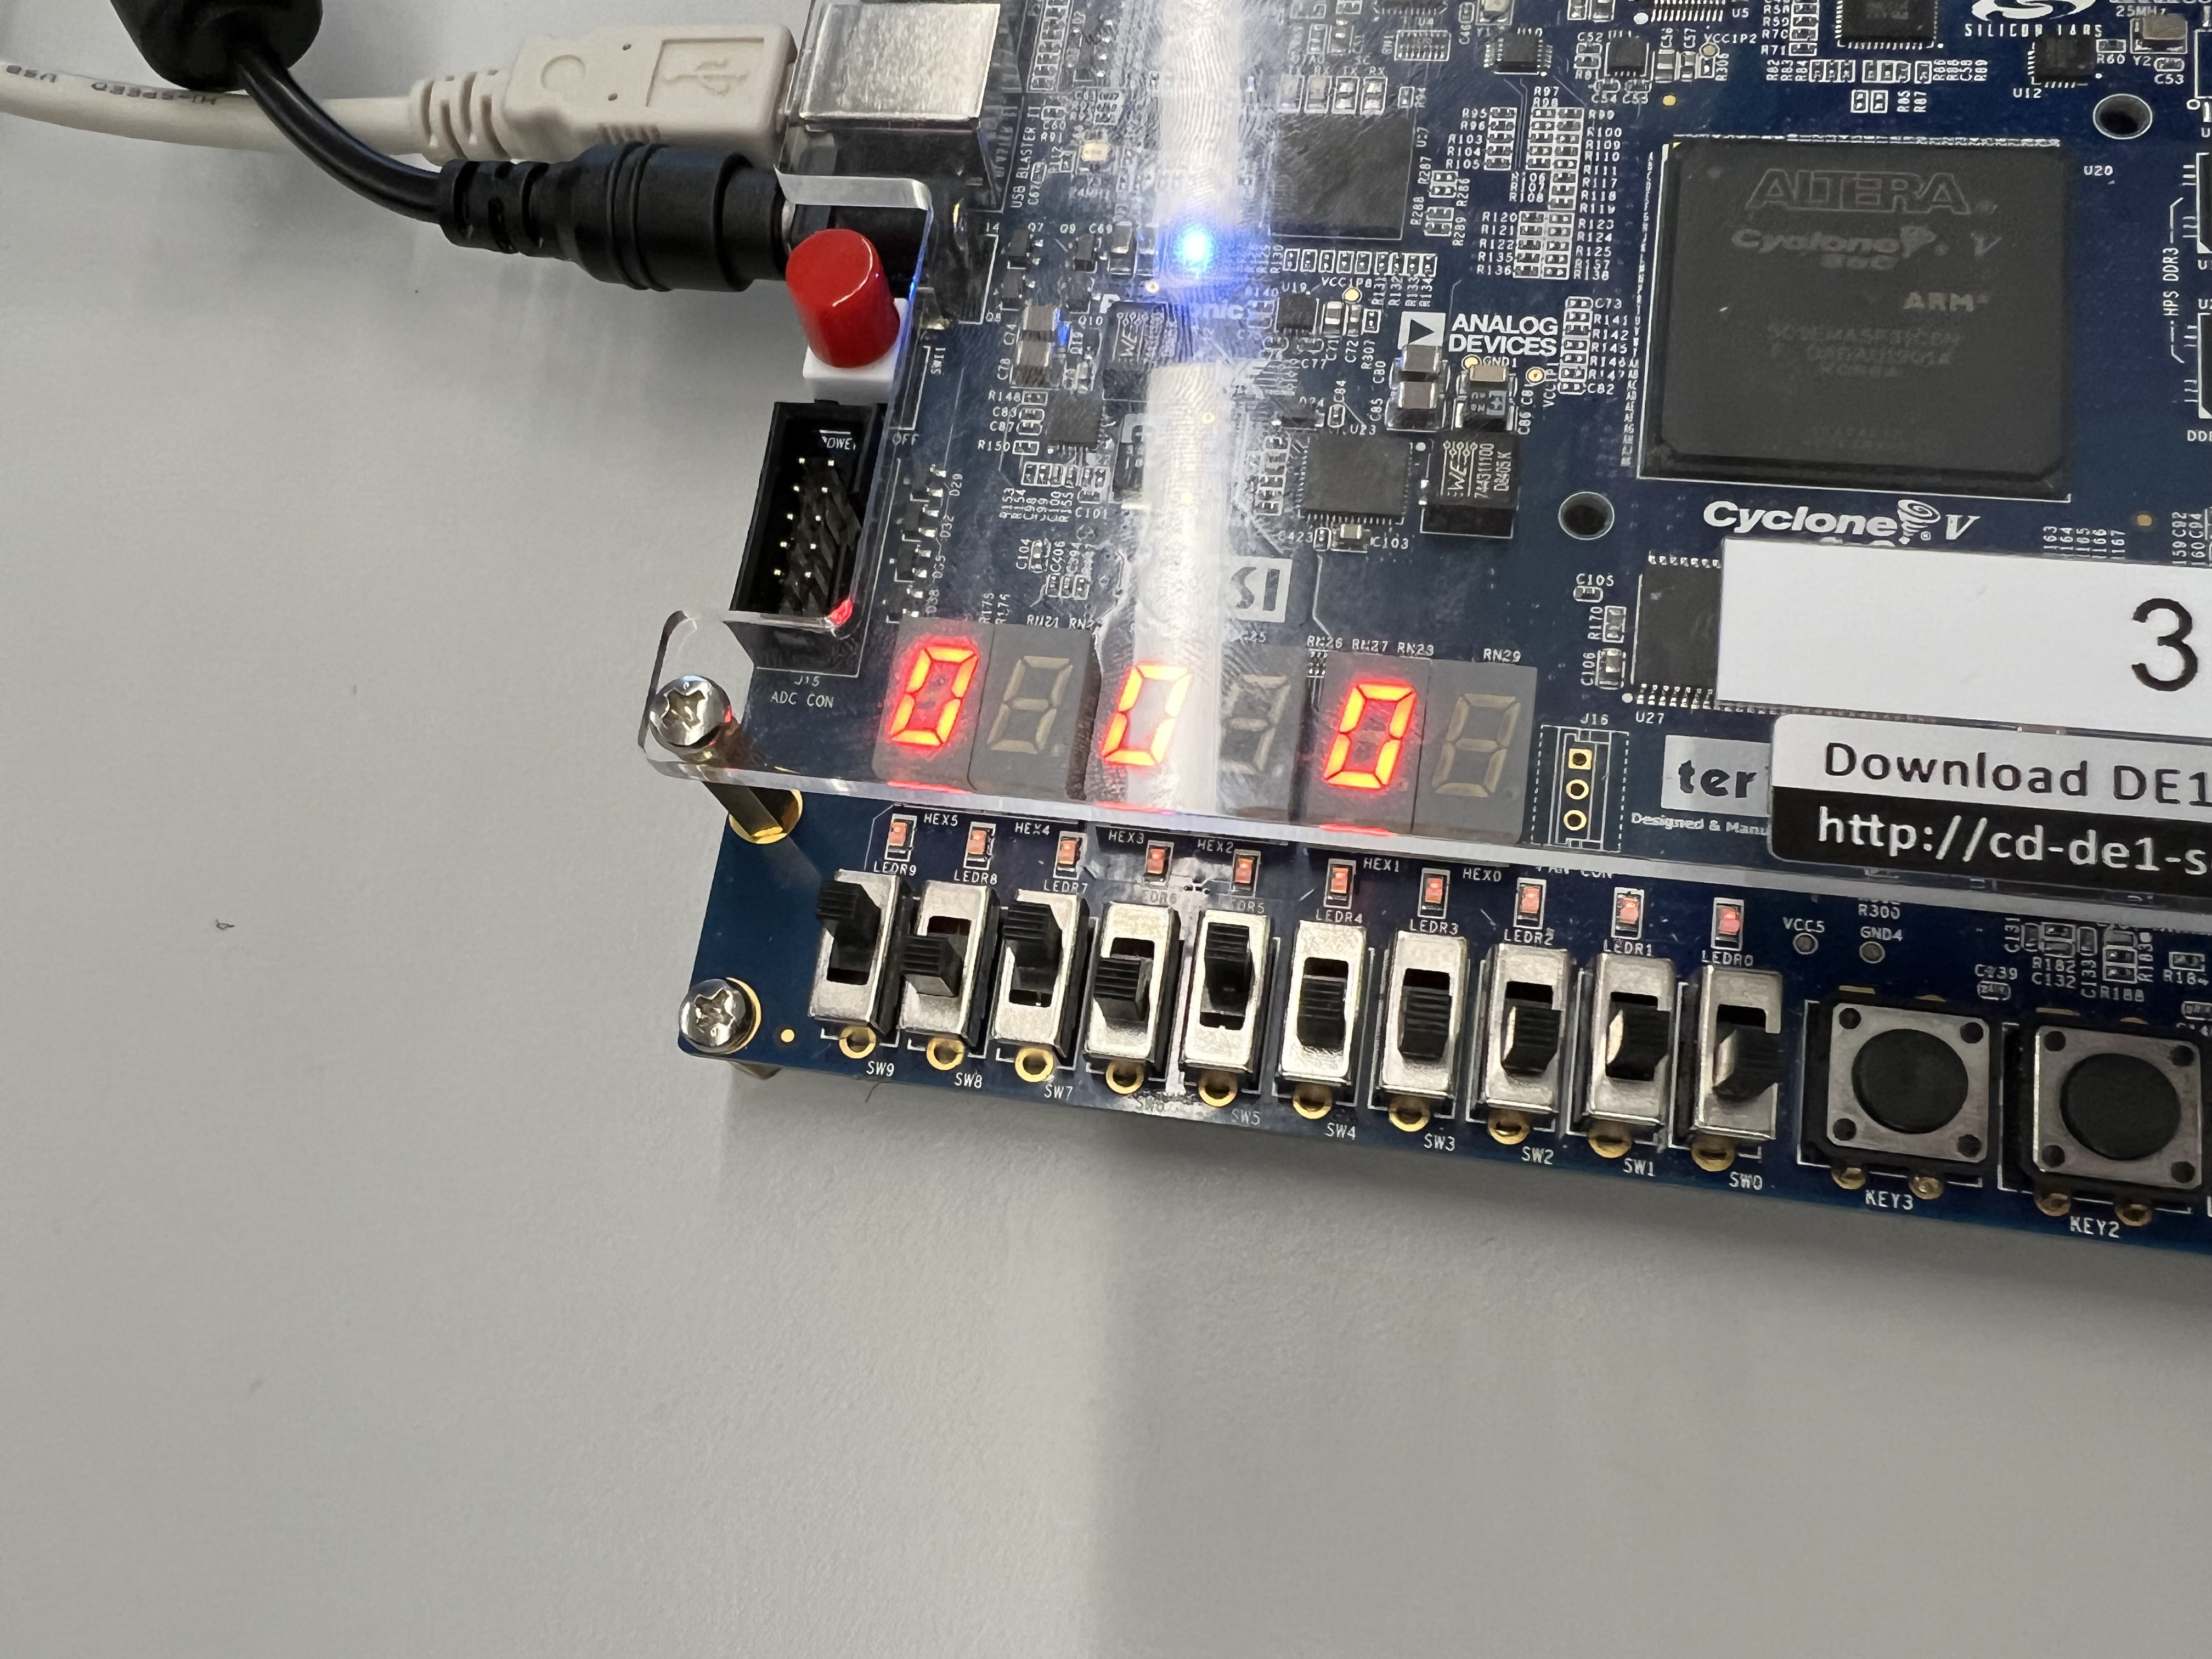
\includegraphics[width=.9\textwidth]{Figures/Three0.jpg}
  \caption{SW[0] is disabled, and SW[5] and SW[7] are enabled}
  \label{fig:16}
\end{figure}

\begin{figure}[H]
  \centering
  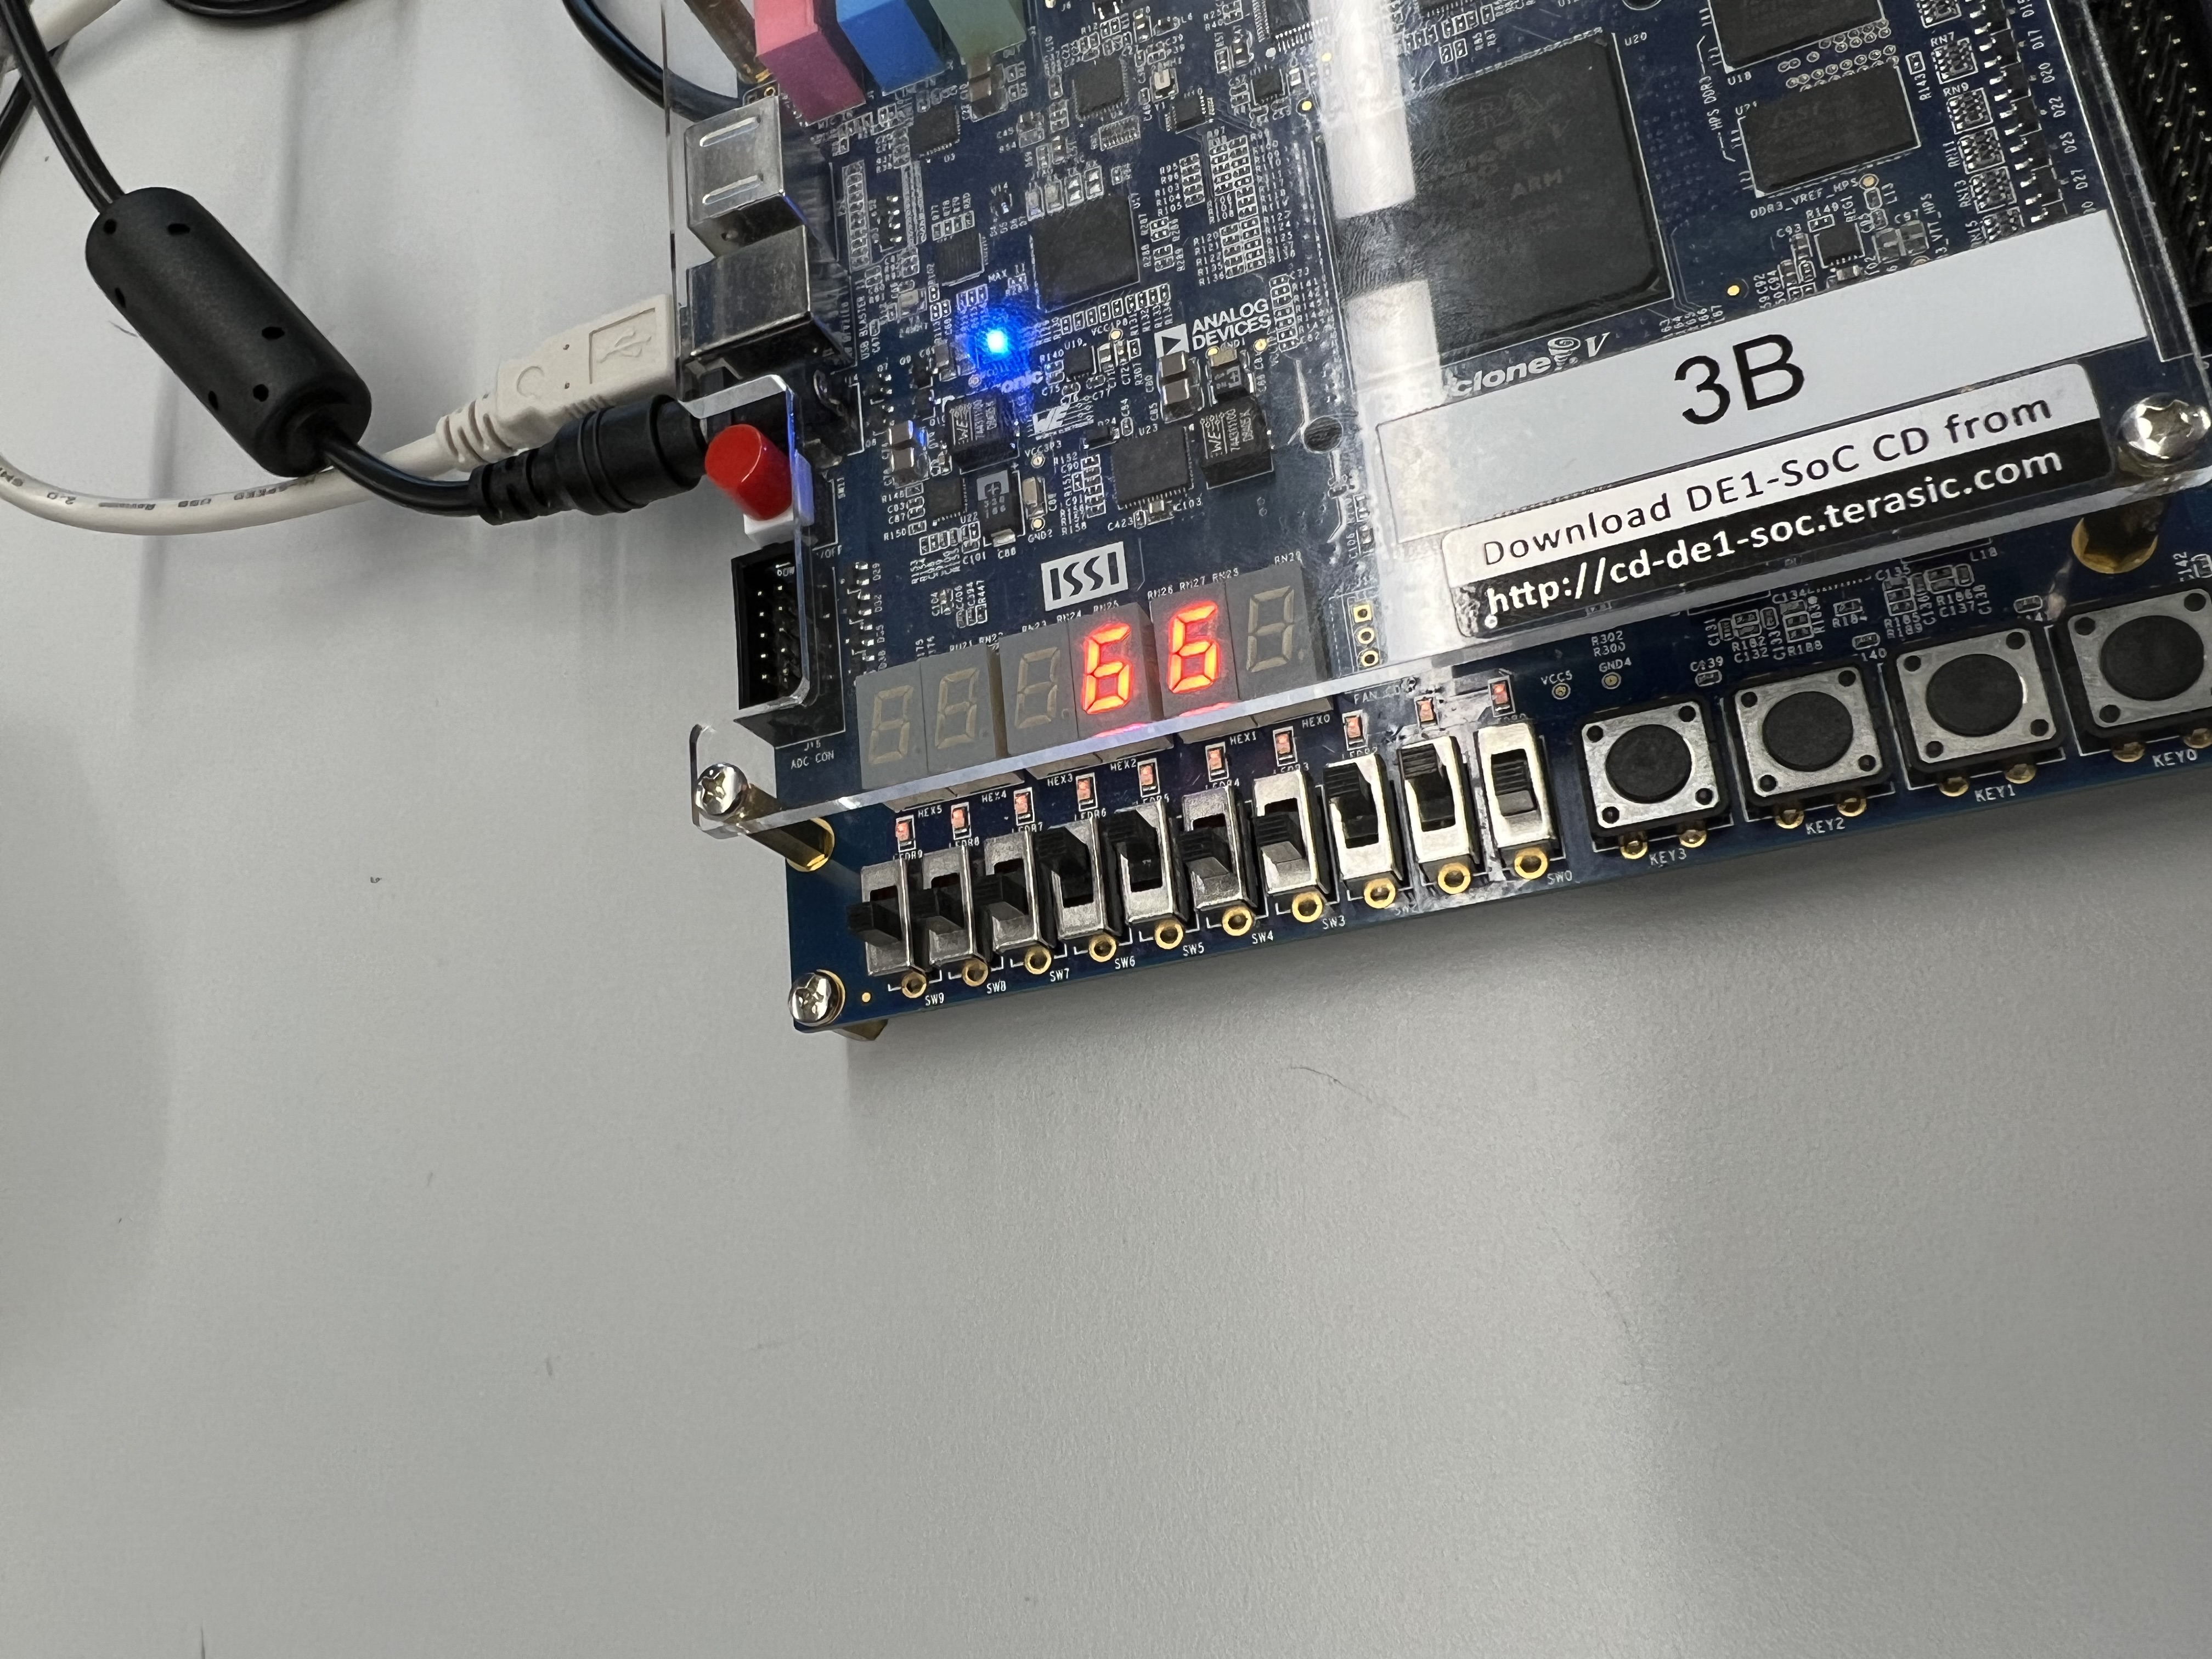
\includegraphics[width=.9\textwidth]{Figures/Two6.jpg}
  \caption{SW[1], SW[2], SW[5], and SW[6] are enabled}
  \label{fig:17}
\end{figure}

\begin{figure}[H]
  \centering
  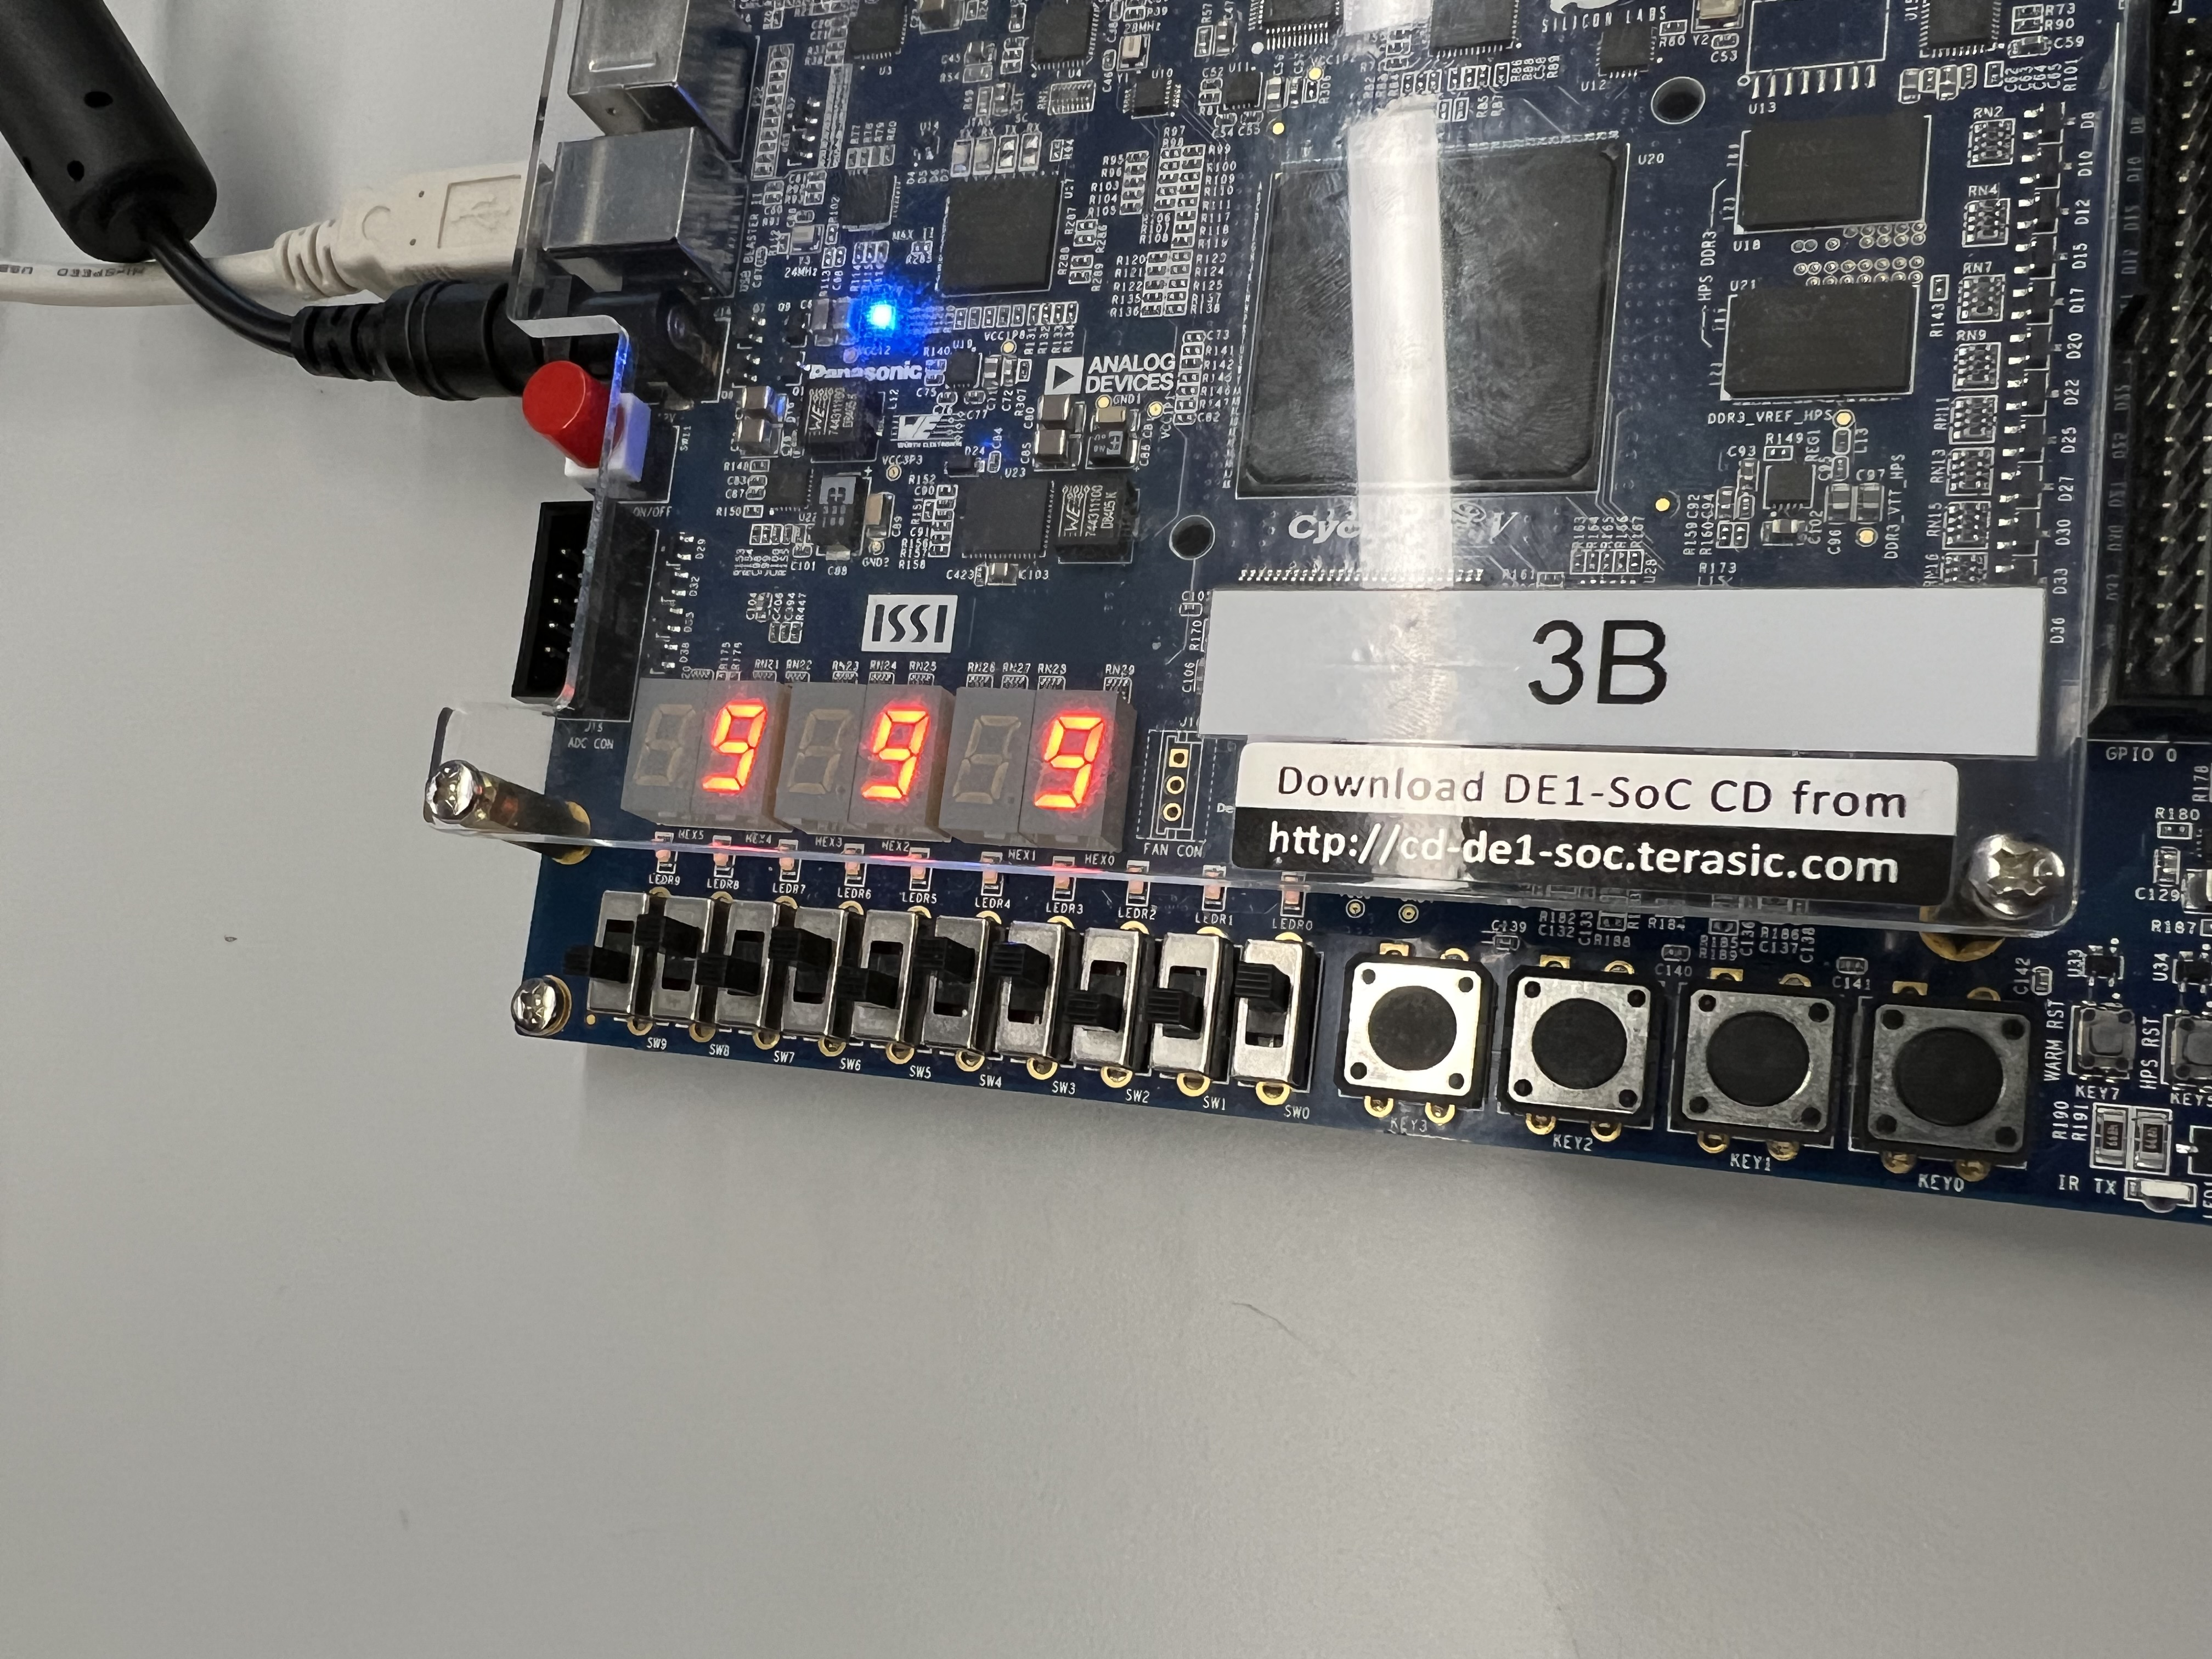
\includegraphics[width=.9\textwidth]{Figures/Three9.jpg}
  \caption{SW[0], SW[3], SW[4], SW[6] and SW[8] are enabled}
  \label{fig:18}
\end{figure}

\begin{figure}[H]
  \centering
  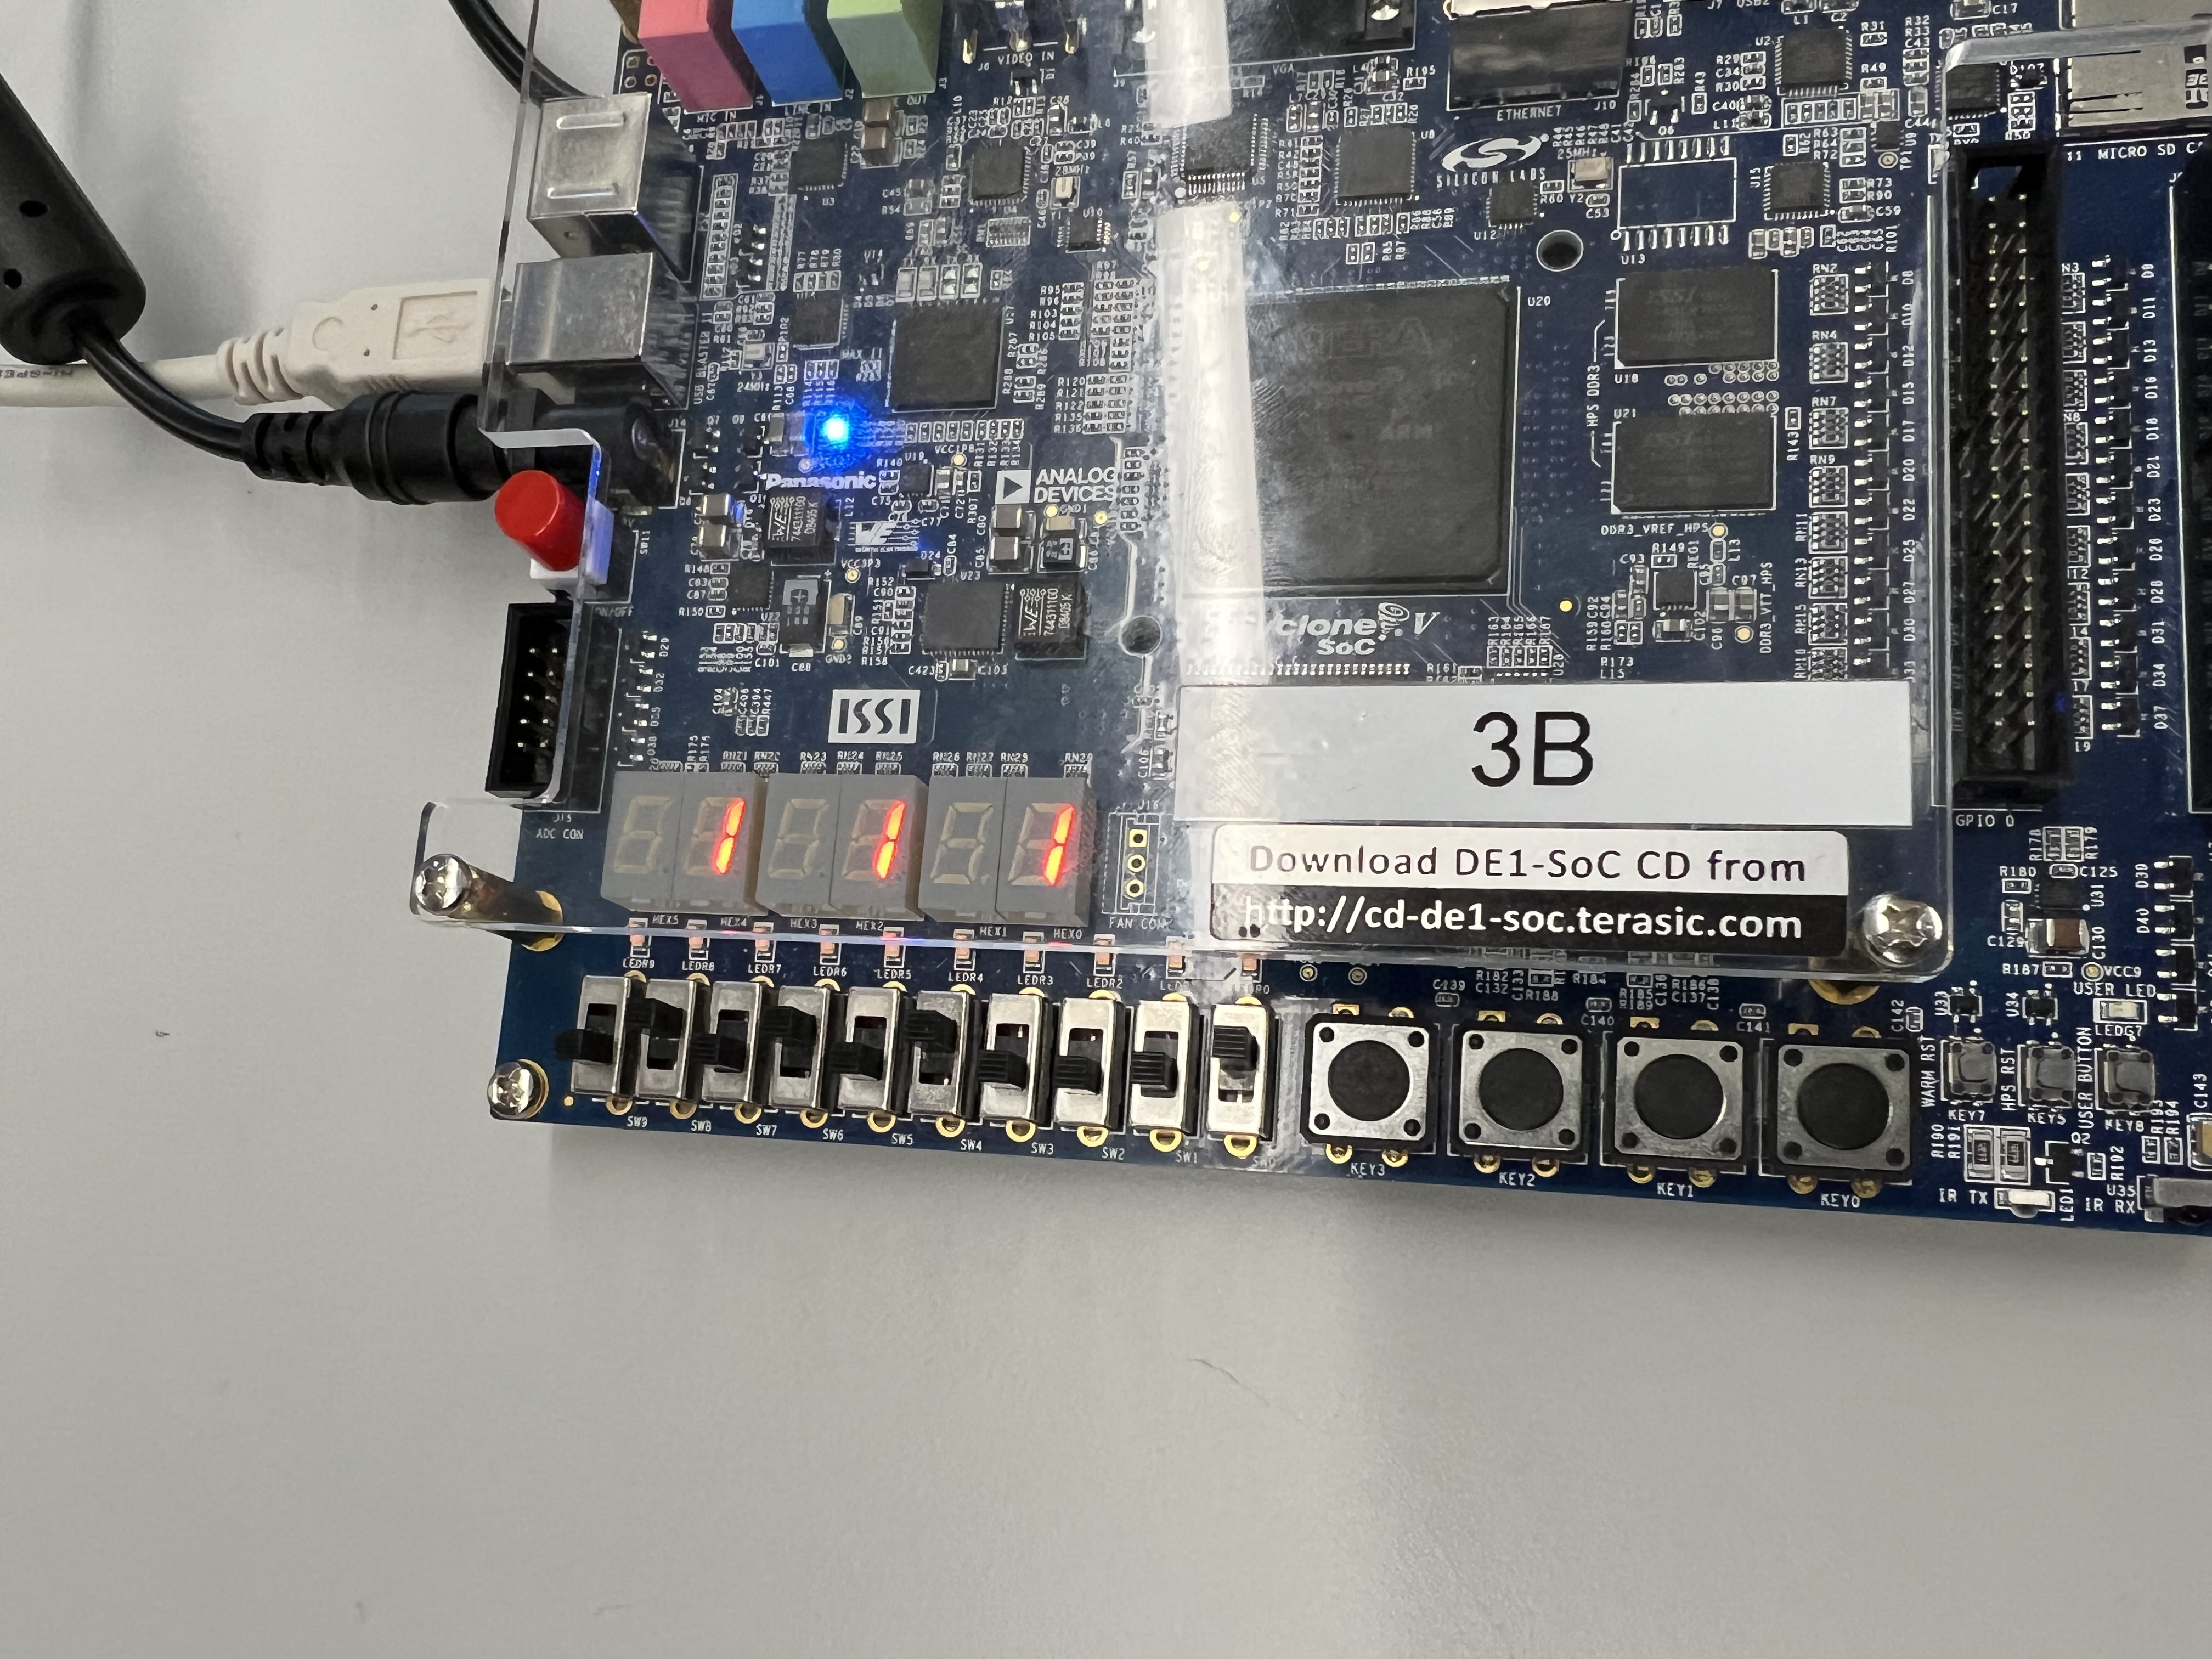
\includegraphics[width=.9\textwidth]{Figures/Three1.jpg}
  \caption{SW[0], SW[4], SW[6] and SW[8] are enabled}
  \label{fig:19}
\end{figure}

\section{Conclusion}

\hspace{.5 in} As a result of the lab, three blocks were successfully constructed: one displaying a digit from 0-9 on the first seven-segment display; another which does the same but allows for the display to be turned on or off; and a third, which allows for all six seven-segment displays to be used, with the option to enable. Of the new concepts introduced, the most important was working with seven-segment displays. In doing so, the user was able to learn how ton best approach seven-segment-display-based problems. 

\end{document}
